\documentclass[11pt,a4paper]{article}

\usepackage[margin=1in]{geometry}
\usepackage{setspace}
\usepackage{amsmath}
\usepackage{booktabs}
\usepackage{longtable}
\usepackage{graphicx}
\usepackage{float}
\usepackage{array}
\usepackage{tabularx}
\usepackage[hidelinks]{hyperref}
\usepackage{caption}
\usepackage{microtype}

\geometry{margin=1in}
\onehalfspacing
\graphicspath{{../figures/}}
\setlength{\parskip}{0.35em}
\setlength{\parindent}{1.2em}
\newcolumntype{L}[1]{>{\raggedright\arraybackslash}p{#1}}
\newcolumntype{C}[1]{>{\centering\arraybackslash}p{#1}}

\begin{document}

\title{\textbf{The Revenue-Surplus Paradox in Arunachal Pradesh: Transfer Dependence, Fiscal Rules, and Frontier-State Growth}}
\author{S.M. Muzammil Afroz\\
Subject: Financial Programming\\
Instructor: M. Parameswaran\\
Centre for Development Studies}
\date{April 2026}
\maketitle

\begin{abstract}
This paper studies Arunachal Pradesh's fiscal health over 1990-91 to 2026-27, with special attention to the recent five-year budget window from 2022-23 to 2026-27. The central empirical puzzle is a revenue-surplus paradox: over the latest five years, the state records revenue surpluses averaging 15.9 percent of GSDP and interest payments averaging only 4.1 percent of revenue expenditure, yet own revenue finances only 18.2 percent of revenue expenditure and central transfers account for 85.9 percent of revenue receipts. A superficial fiscal-health reading would treat the state as unusually strong. The paper argues instead that headline strength is transfer-produced rather than autonomous. The analysis combines the RBI State Finance Database, current-price GSDP data, the 2026-27 Arunachal Pradesh budget packet, PRS budget material, and the 15th and 16th Finance Commission reports. It makes four contributions. First, it situates Arunachal Pradesh within the Indian fiscal federalism, North-Eastern and Himalayan states, and Finance Commission transfer literatures. Second, it extends the four core fiscal indicators into a long-run fiscal-history figure. Third, it fixes the own-tax buoyancy exercise by reporting unit-root and Engle-Granger diagnostics; the coefficient is informative but the cointegration evidence is not strong enough to support a causal long-run claim. Fourth, it treats the accounting gap between the broad PRS-style fiscal deficit, which reaches 10.5-11.0 percent of GSDP in 2025-26 and 2026-27, and the official deficit of 1.6-1.7 percent as the paper's main methodological finding. The gap arises because 50-year interest-free central capex loans under SASCI are excluded from the operative borrowing-ceiling calculation. Arunachal Pradesh is therefore best described as headline-strong but structurally transfer-dependent.
\end{abstract}

\tableofcontents
\newpage

\section{Introduction}

A standard fiscal-health exercise for an Indian state begins with four indicators: revenue deficit as a share of GSDP, fiscal deficit as a share of GSDP, primary deficit as a share of GSDP, and interest expenditure as a share of revenue expenditure. For Arunachal Pradesh, those ratios are informative but incomplete. The state rarely appears fiscally weak on the headline indicators. Revenue balance is positive, interest burden is low, and the official budget presentation reports only modest fiscal deficits in the latest years. Yet the state remains overwhelmingly dependent on central transfers.

That combination motivates the paper's research question: what exactly do ``healthy'' fiscal ratios mean in a frontier state whose own resource base is narrow and whose expenditure capacity is supported by large transfers from the Centre? The answer developed here is that Arunachal Pradesh exhibits a \emph{revenue-surplus paradox}. It appears fiscally strong under the headline ratios, but the underlying strength is not self-financed. It is produced by transfers, concessional borrowing windows, and a fiscal architecture that allows the state to spend without building a correspondingly strong own-revenue base.

The paper therefore does two things. First, it completes a five-year fiscal table with the latest available official 2026-27 budget documents. Second, it turns the exercise into a broader argument about transfer dependence, fiscal-rule interpretation, and the relationship between fiscal structure and the state's growth pattern. The novelty is not another descriptive state-budget summary. It is the demonstration that Arunachal Pradesh can simultaneously show large revenue surpluses, low interest burden, weak own-resource capacity, high capital spending, and limited structural transformation.

\section{Research Question and Contribution}

The main contribution is conceptual rather than purely computational. A standard fiscal-health reading would conclude that Arunachal Pradesh is prudent because it runs revenue surpluses and keeps interest payments low. This paper argues that such a conclusion is incomplete unless fiscal autonomy is studied alongside fiscal balances. Four extensions generate the research contribution.

First, the paper places the four core ratios inside a longer-run fiscal-dependence framework using the RBI State Finance Database. Second, it provides a substantive literature review around Indian fiscal federalism, transfer design, special-category and North-Eastern/Himalayan state fiscal structure, and Finance Commission criteria. Third, it reconciles two deficit concepts that now coexist in the 2026-27 budget context: the broad PRS-style fiscal deficit and the smaller official state-budget deficit after deducting central capex loans. Fourth, it links fiscal structure to the state's service-heavy, transfer-supported growth pattern. The result is a unified frontier-state interpretation of growth and public finance.

\section{Literature Review}

\subsection{Fiscal federalism and vertical imbalance}

The starting point is the Indian fiscal federalism literature. Rao and Singh argue that India assigns large expenditure responsibilities to states while retaining major revenue powers at the Union level, producing persistent vertical fiscal imbalance that must be closed by Finance Commission devolution, grants, and other central transfers \cite{rao_singh_2005}. That argument is directly relevant to Arunachal Pradesh because the state is not merely a small administrative unit with temporary fiscal dependence. It is an extreme case of the structural mismatch built into the federal system. The state must finance public administration, roads, social services, and border-area infrastructure across difficult terrain, but its own tax base is narrow.

Rao's earlier work on state finances emphasises that state-level fiscal stress in India cannot be understood only from aggregate deficit ratios \cite{rao_2002}. The composition of revenue, the buoyancy of transfers, the burden of salaries and interest, and the crowding-out of capital expenditure all matter. This paper follows that logic. A revenue surplus is treated as an accounting result to be explained, not as sufficient evidence of fiscal autonomy. In Arunachal Pradesh, revenue surplus is large because transfers are large relative to current expenditure. That is different from the revenue surplus of a high-capacity industrial state.

The vertical-imbalance framework also explains why headline rules can be misleading. If a state depends heavily on central transfers, its budget balance can improve or deteriorate because of changes in the transfer formula rather than because of changes in state effort. This is why the paper places the headline ratios beside fiscal dependence, own revenue relative to revenue expenditure, and the composition of grants.

\subsection{Transfer design, incentives, and fiscal discipline}

The international transfer-design literature gives the second pillar. Bird and Smart argue that intergovernmental grants should be judged not only by whether they equalise fiscal capacity but also by the incentives they create for own-source revenue effort and expenditure choice \cite{bird_smart_2002}. Equalising transfers are necessary when poor or geographically disadvantaged jurisdictions cannot provide minimum public services, but poorly designed transfers can soften budget constraints. The relevant question is therefore not whether Arunachal Pradesh should receive transfers. It should. The question is whether the transfer system also encourages a gradual strengthening of own revenue capacity and expenditure efficiency.

Bhatt and Scaramozzino bring this question to the Indian state setting. Their empirical work links federal transfers, state domestic product, and state fiscal discipline, and highlights the risk that gap-filling transfers can accommodate deficits rather than discipline them \cite{bhatt_scaramozzino_2015}. This paper's empirical result is not identical to theirs. Arunachal Pradesh does not display an ordinary chronic revenue-deficit problem in the latest window. Instead, it displays the opposite surface pattern: high revenue surplus. But the underlying issue is similar. When transfers dominate the revenue base, standard deficit indicators become partly endogenous to the transfer system.

Rangarajan and Srivastava focus on the institutional relation between transfers and fiscal responsibility \cite{rangarajan_srivastava_2011}. Their work is important here because Arunachal Pradesh's 2026-27 fiscal interpretation depends on the boundary between ordinary borrowing and special central capital loans. If fiscal rules are evaluated using a deficit number that excludes a large concessional loan window, then rule compliance and broader financing dependence can diverge. The paper's deficit-reconciliation section is therefore not a mechanical footnote. It is an application of the fiscal-responsibility literature to a specific contemporary accounting issue.

\subsection{Special category states and the North-Eastern/Himalayan fiscal problem}

The special-category and North-Eastern/Himalayan state literature adds a third layer. The 15th Finance Commission explicitly discusses the fiscal disabilities of North-Eastern and Himalayan states, including small revenue bases, high infrastructure costs, and the need to account for forest and ecological services in the devolution formula \cite{fifteenth_fc_2020}. Arunachal Pradesh fits this category strongly: sparse settlement, forest cover, border location, difficult terrain, and weak manufacturing depth all raise public-spending need while limiting the tax base.

The 16th Finance Commission updates this context. Its framework retains a 41 percent vertical devolution share to states, changes horizontal weights by giving 42.5 percent to income distance, 17.5 percent to 2011 population, 10 percent to demographic performance, 10 percent to area, 10 percent to forest, and 10 percent to contribution to GDP, while dropping the explicit tax-and-fiscal-effort criterion used by the 15th Finance Commission \cite{sixteenth_fc_2026,prs16fc}. For Arunachal Pradesh, the practical implication is sharp: its inter-se devolution share falls from 1.76 percent under the 15th Finance Commission to 1.35 percent under the 16th. That decline is central to the transfer-shock simulation in this paper.

The 16th Finance Commission also reports that North-Eastern and Himalayan states remain heavily dependent on devolution and Union transfers, and it identifies Arunachal Pradesh as a high-transfer, high-capital-expenditure state. This matters because the policy question is not simply whether Arunachal Pradesh spends too much. The evidence suggests it spends a large share on capital outlay, helped by special central capital support. The deeper question is whether this capital push is building an economy that can later carry more of its own fiscal load.

\subsection{FRBM rules, capital expenditure, and the quality of adjustment}

The fiscal-rule literature warns against treating numerical compliance as the whole story. Chakraborty and Dash show that rule-based fiscal consolidation in Indian states must be evaluated together with development spending and the quality of adjustment \cite{chakraborty_dash_2013}. This is directly relevant to Arunachal Pradesh because the state combines low official fiscal deficit with large capital outlay and large central capex loans. A strict deficit interpretation could understate financing dependence, while a strict deficit criticism could understate the developmental logic of concessional capital finance.

The RBI's \emph{State Finances: A Study of Budgets} series provides the operational framework for this kind of analysis: revenue balance, gross fiscal deficit, interest burden, committed expenditure, debt, and capital outlay are complementary indicators rather than substitutes \cite{rbi_state_finances_2023}. The present paper follows that multi-indicator approach. The four core ratios are necessary, but they are not sufficient for a publishable fiscal diagnosis.

\subsection{Arunachal Pradesh-specific evidence}

The Arunachal Pradesh-specific literature reinforces the same conclusion. The Rajiv Gandhi University evaluation prepared for the 15th Finance Commission documents that Arunachal Pradesh has long shown revenue surpluses and low own-tax capacity, while central transfers account for a very large share of aggregate revenue \cite{nayak_rgu_2019}. It also highlights hydro-power potential, administrative size, dependence on centrally sponsored schemes, and the importance of expanding own non-tax revenue. The present paper updates that earlier diagnosis to the 2026-27 budget environment and adds three new elements: the 16th Finance Commission share reduction, the central capex-loan reconciliation, and the long-run link between fiscal dependence and the state's broader growth pattern.

This literature review leads to the paper's core proposition. In a frontier state such as Arunachal Pradesh, fiscal health must be read through three lenses at once: headline balances, transfer dependence, and fiscal-rule accounting. A strong revenue balance is meaningful, but it is not equivalent to fiscal autonomy.

\section{Institutional and Fiscal Background}

Arunachal Pradesh is a geographically difficult, sparsely populated border state with high logistics costs and a historically weak industrial base. These characteristics matter for both growth and fiscal analysis. They raise the cost of infrastructure, increase the role of public administration and transfers, and limit the pace at which the state can widen its own tax base. In such a setting, fiscal indicators should not be read in the same way as they would be for a large industrial state.

The fiscal-rule context also matters. The Arunachal Pradesh Fiscal Responsibility and Budget Management framework formally anchors fiscal discipline, but the 2026-27 budget documents show that interpretation depends on how central capex loans are treated. The broader deficit concept counts those loans in net borrowing; the official state-budget presentation nets them out for the operative fiscal-deficit discussion. The state's own FRBM statement notes that the normal net-borrowing limit is 3 percent of GSDP for 2026-27 to 2030-31 and that Union on-lending under the Special Assistance to States for Capital Investment (SASCI) is over and above that limit. This accounting distinction materially changes the reported deficit ratio and therefore the substantive interpretation of compliance and sustainability.

\section{Data and Document Sources}

The main historical fiscal backbone is the RBI State Finance Database. It remains the principal source for long-run receipts, expenditure, grants, own revenue, and transfer dependence. However, the latest official budget year studied here extends to 2026-27, while the RBI extract used for the historical database ends at 2025-26 Budget Estimates. Accordingly, the paper adds a narrow official top-up layer from the 2026-27 Arunachal budget packet.\footnote{Official Arunachal budget portal: \url{https://www.arunachalbudget.in/}.}

The official documents used are the 2026-27 \emph{Budget at a Glance}, \emph{Annual Financial Statement}, \emph{Fiscal Responsibility \& Budget Management} statement, \emph{Demands for Grants}, and \emph{Budget Speech}. For current policy interpretation and deficit reconciliation, the paper also uses the PRS Arunachal Pradesh Budget Analysis 2026-27 and the PRS summary of the 16th Finance Commission report for 2026-31. These files are stored locally in \texttt{Data/Project2\_Budget\_Documents/}.

This hybrid design keeps the RBI database as the core quantitative source and uses the official budget packet only where the RBI data do not yet provide the final budget year or where the deficit definition must be reconciled explicitly.

\begin{table}[H]
\centering
\caption{Data validation checks for the extended fiscal dataset}
\small
\begin{tabular}{L{5.2cm}L{6.3cm}C{1.8cm}}
\toprule
Check & Result & Status \\
\midrule
RBI Arunachal account coverage & Account data available from 1990-91 to 2023-24 & Pass \\
Required RBI budget heads & Revenue, own tax, central taxes, grants, revenue expenditure, capital outlay, and net capital expenditure heads found in both Arunachal and all-state files & Pass \\
2026-27 GSDP denominator & Rs 41,314 crore, cross-checked against Budget at a Glance text & Pass \\
Comparator GSDP coverage & All six comparator states have 2023-24 current-price GSDP & Pass \\
\bottomrule
\end{tabular}
\caption*{\footnotesize Notes: The earlier local typo `41,341' for 2026-27 GSDP was corrected to the Budget at a Glance value of Rs 41,314 crore. The correction does not alter the rounded headline ratios in the fiscal-indicator table.}
\end{table}

\section{Construction of the Four Core Fiscal Indicators}

All figures are expressed in rupees crore. Revenue balance is defined as revenue receipts minus revenue expenditure. A positive value implies revenue surplus. Interest burden is interest expenditure divided by revenue expenditure.

Fiscal balance and primary balance require more care. For 2022-23 and 2023-24, the paper constructs a state-budget-style fiscal balance from the RBI database by combining revenue expenditure, capital expenditure net of public accounts, loan recoveries, and loans from the Centre. For 2024-25 actual, 2025-26 revised, and 2026-27 budget estimates, the paper uses the official 2026-27 budget documents and then separates two measures:

\begin{enumerate}
\item the \textbf{broad fiscal deficit}, which aligns with the PRS-style `net expenditure minus net receipts' concept, and
\item the \textbf{official fiscal deficit}, which deducts central capex loans in line with the state-budget presentation.
\end{enumerate}

Primary balance is then derived as fiscal balance plus interest payments. The official state-budget presentation is treated as the baseline for the headline table, while the broad deficit measure is retained as a robustness and interpretation check.

\section{Long-Run Fiscal Structure}

The five-year table should be read against a longer history. Figure \ref{fig:longrun} extends the four core indicators from 1990-91 to 2026-27. The historical fiscal and primary balances are shown on the broad state-budget concept before deducting central capex loans; the official capex-loan adjustment is then handled separately in the reconciliation section. This avoids mixing a recent fiscal-rule convention with older RBI series.

\begin{figure}[H]
\centering
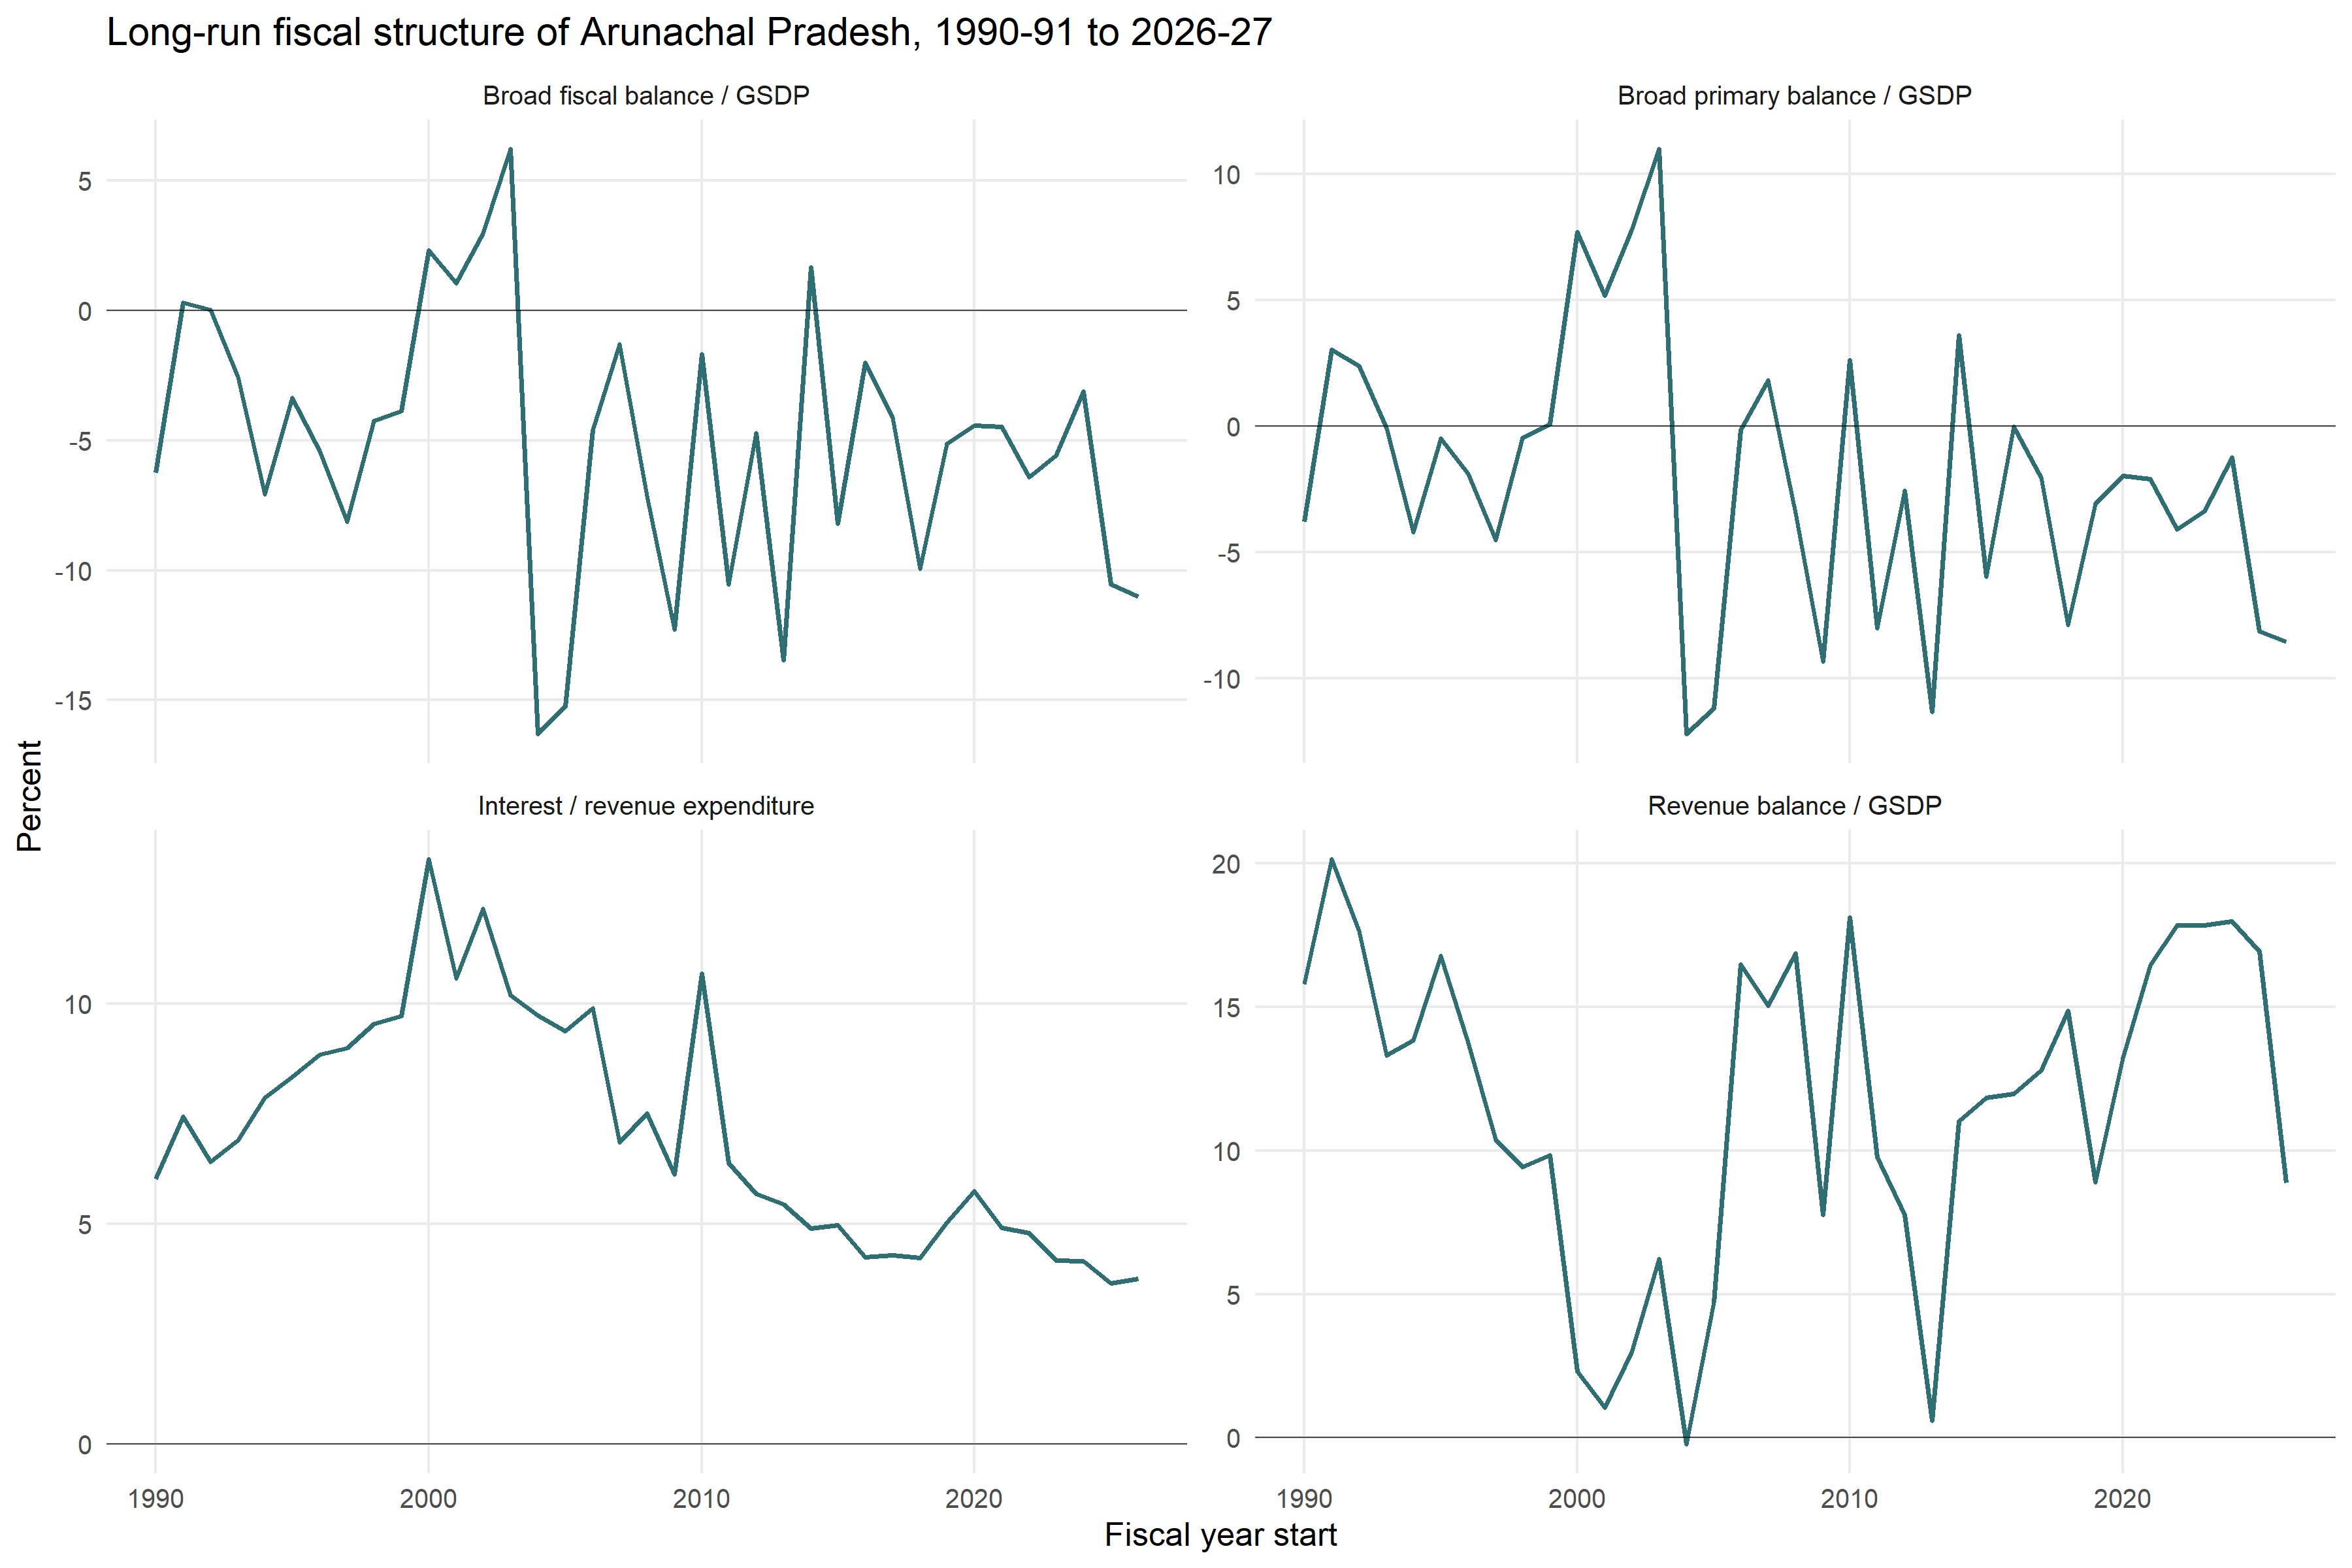
\includegraphics[width=0.96\textwidth]{fig22_project2_longrun_core_indicators.png}
\caption{Long-run fiscal structure of Arunachal Pradesh, 1990-91 to 2026-27}
\label{fig:longrun}
\end{figure}

Three patterns stand out. First, revenue balance has usually been positive, but it is volatile and transfer-sensitive. The sharp fall in 2026-27 is not a collapse into revenue deficit; it is a compression of the surplus after the 16th Finance Commission devolution-share reduction. Second, the broad fiscal and primary balances are much more volatile than the revenue balance. This reflects the importance of capital expenditure and central capital support in a frontier state. Third, interest burden has trended downward from the high levels around 2000-01 and now sits below 5 percent of revenue expenditure. This is genuine fiscal comfort, but it coexists with weak own-resource capacity.

\begin{table}[H]
\centering
\caption{Core fiscal indicators, Arunachal Pradesh, 2022-23 to 2026-27}
\small
\begin{tabular}{L{1.7cm}C{1.8cm}C{2.0cm}C{2.1cm}C{1.8cm}}
\toprule
Year & Revenue balance / GSDP & Official fiscal balance / GSDP & Official primary balance / GSDP & Interest / Rev. exp. \\
\midrule
2022-23 & 17.8 & -2.0 & 0.3 & 4.8 \\
2023-24 & 17.8 & 0.5 & 2.8 & 4.2 \\
2024-25 & 18.0 & 2.0 & 3.9 & 4.2 \\
2025-26 & 16.9 & -1.6 & 0.8 & 3.6 \\
2026-27 & 8.9 & -1.7 & 0.8 & 3.8 \\
\bottomrule
\end{tabular}
\caption*{\footnotesize Notes: Positive fiscal and primary balances denote surplus. The 2024-25 to 2026-27 rows use official budget-document top-up values; 2025-26 is Revised Estimate and 2026-27 is Budget Estimate.}
\end{table}

\section{Extended Fiscal Indicators and Transfer Dependence}

The headline ratios are only the first layer. The more revealing indicators are the fiscal-dependence ratio, own revenue relative to revenue expenditure, own tax as a share of own revenue, and capital outlay relative to expenditure.

The long-run fiscal-dependence ratio remains extremely high. In the most recent five-year window, central transfers account for 83.1 to 87.2 percent of revenue receipts. The latest official 2026-27 budget mix is especially revealing: central transfers amount to 83.1 percent of revenue receipts, while own revenue finances only 19.2 percent of revenue expenditure. Even in the latest budget, the state is far from fiscally self-financing.

\begin{table}[H]
\centering
\caption{Transfer dependence and own-revenue weakness in the recent budget window}
\small
\begin{tabular}{L{1.7cm}C{1.7cm}C{1.8cm}C{1.8cm}C{1.8cm}}
\toprule
Year & Fiscal dependence & Own rev. / rev. exp. & Own tax / own rev. & CSS grants \\
\midrule
2022-23 & 86.3 & 18.7 & 68.7 & 2,848 \\
2023-24 & 86.5 & 18.0 & 75.6 & 3,371 \\
2024-25 & 87.2 & 17.8 & 72.9 & 3,051 \\
2025-26 & 86.3 & 17.2 & 69.5 & 4,028 \\
2026-27 & 83.1 & 19.2 & 69.8 & 4,200 \\
\bottomrule
\end{tabular}
\caption*{\footnotesize Notes: Fiscal dependence is central tax devolution plus grants divided by revenue receipts. CSS grants are Rs crore. The 2024-25 to 2026-27 rows use the Annual Financial Statement and PRS Budget Analysis top-up.}
\end{table}

These numbers are the core evidence for the revenue-surplus paradox. Revenue surplus does not mean the state can finance itself. It means transfers are large relative to revenue expenditure. Own revenue remains too small to support any claim of autonomous fiscal strength. The state is not merely borrowing little; it is borrowing little because transfers and special borrowing windows dominate the funding structure.

\begin{figure}[H]
\centering
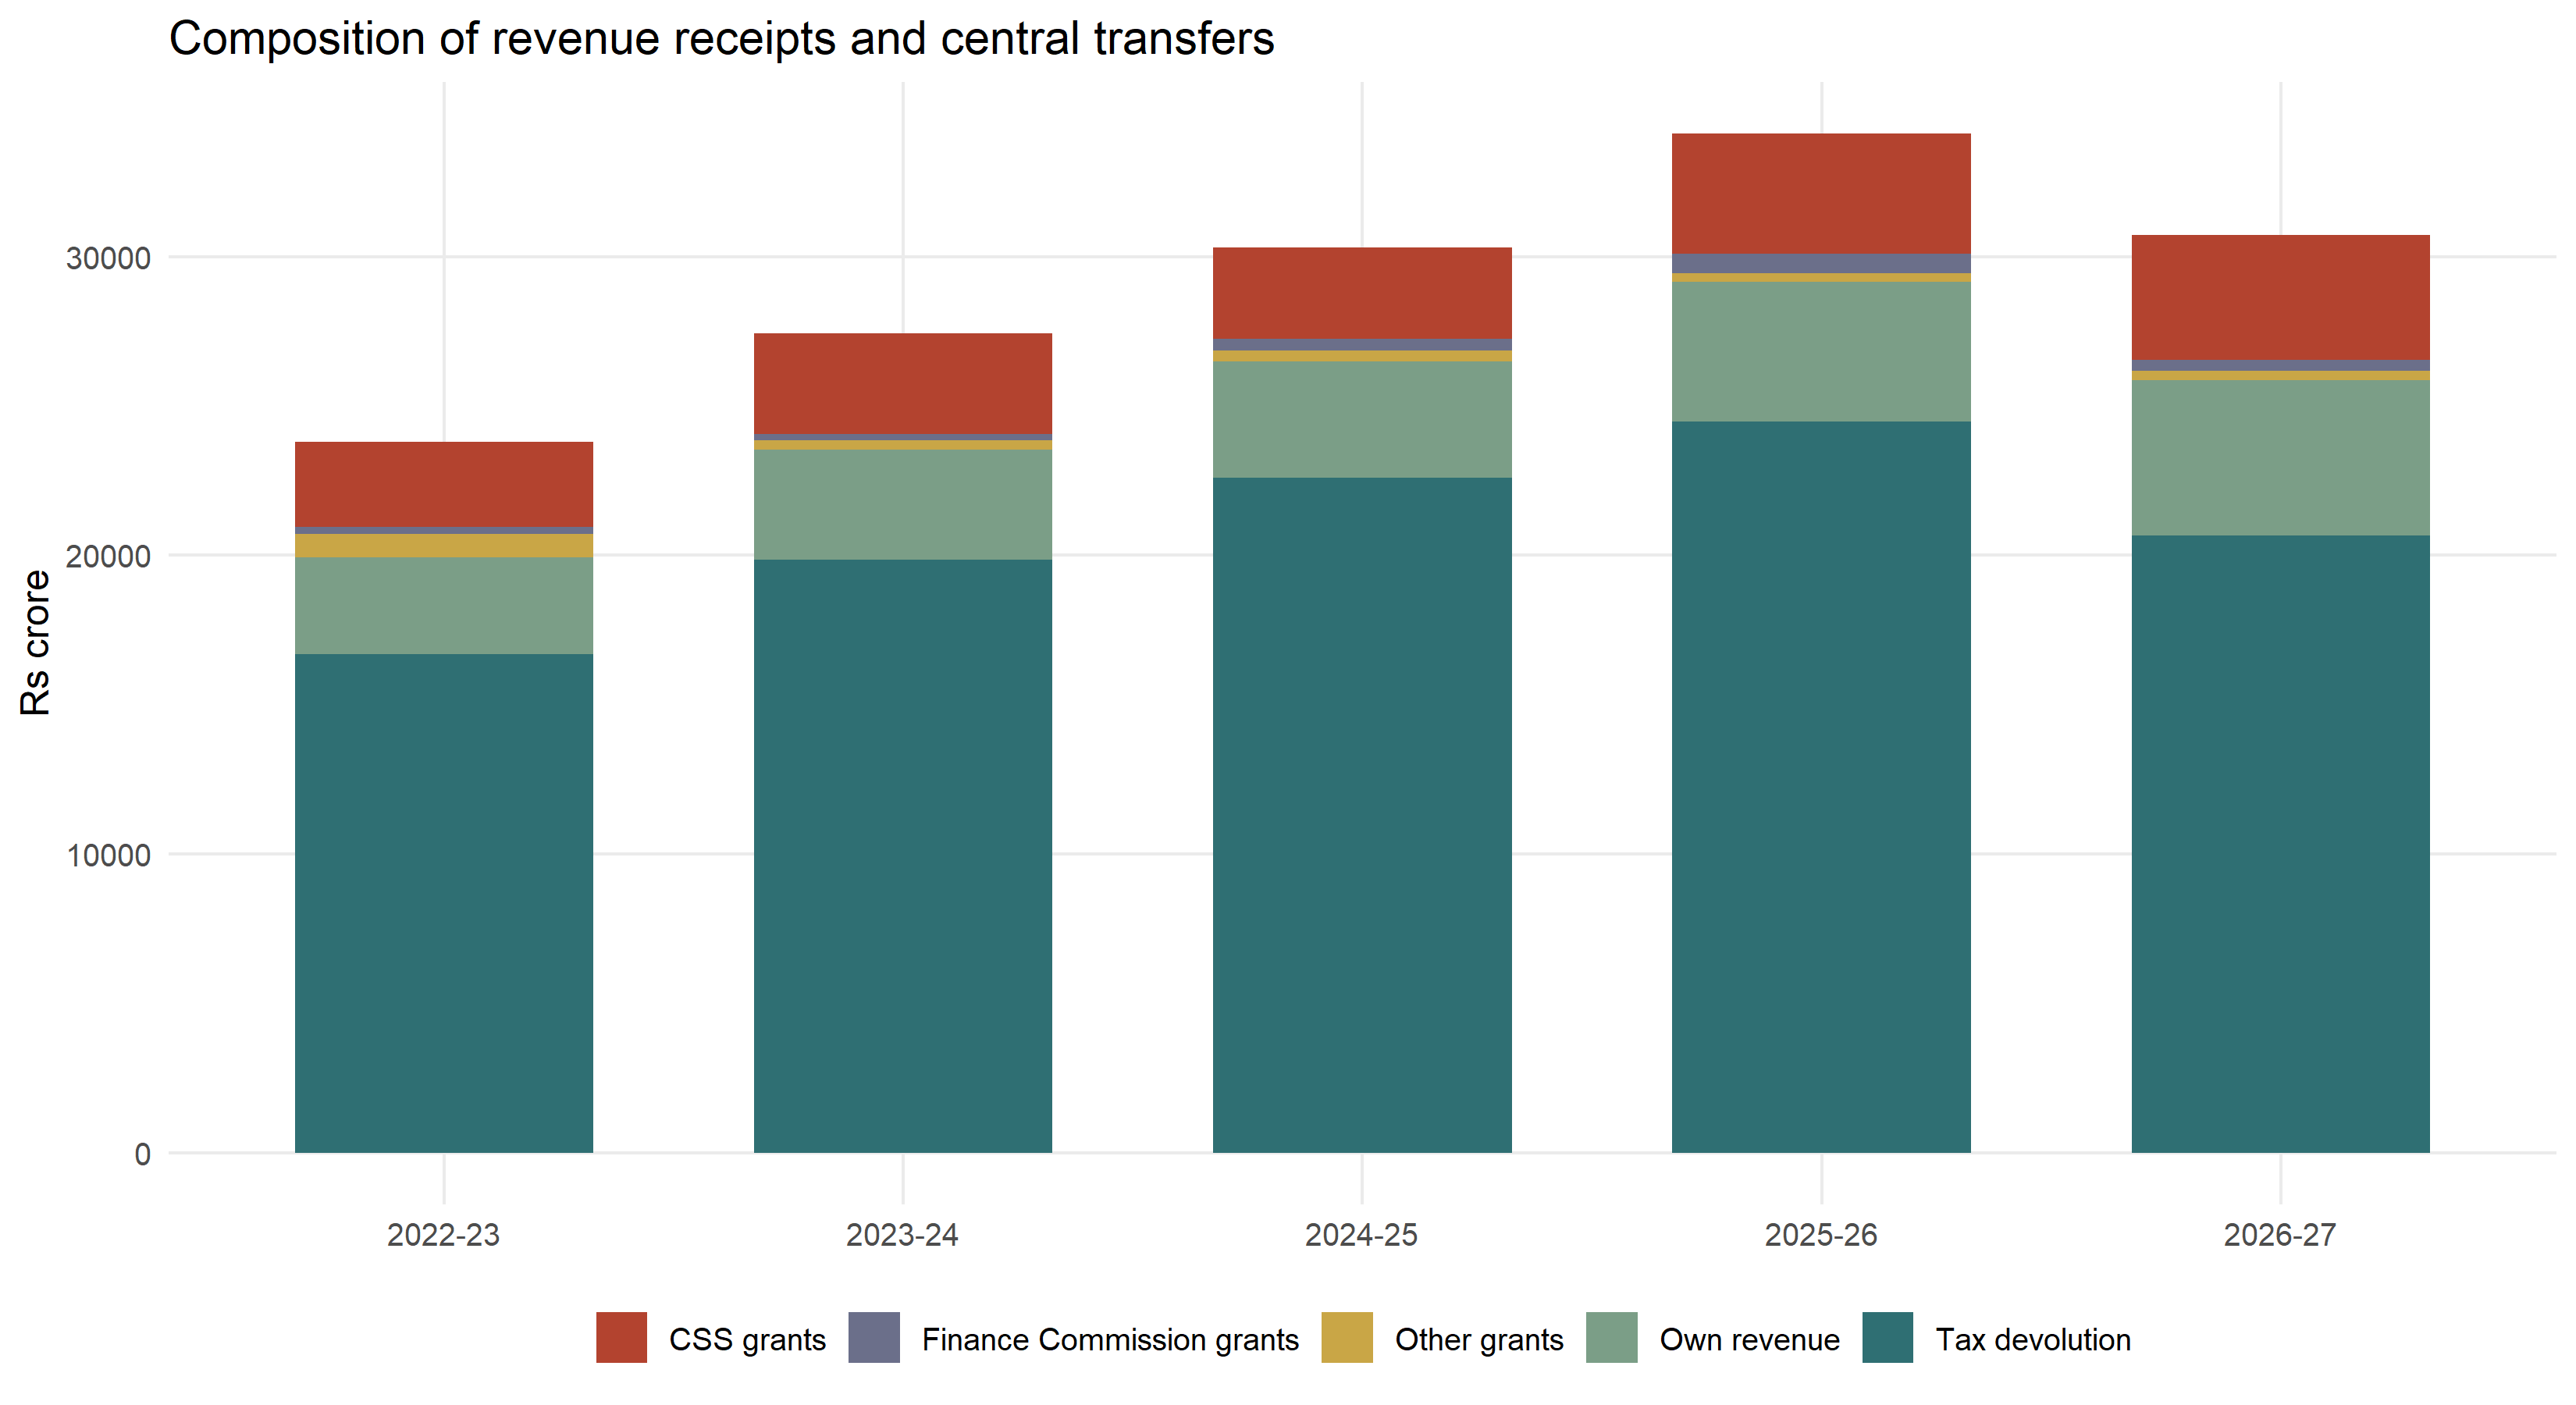
\includegraphics[width=0.88\textwidth]{fig24_project2_transfer_breakdown.png}
\caption{Composition of revenue receipts and central transfers}
\label{fig:transferbreakdown}
\end{figure}

\section{Results}

\subsection{Headline fiscal health}

The five-year table shows three robust features. First, revenue balance is large and always positive, though it declines sharply to 8.9 percent of GSDP in 2026-27. Second, interest burden is low throughout, remaining under 5 percent of revenue expenditure. Third, the official fiscal balance oscillates around zero rather than showing chronic stress. Under the official state-budget presentation, the state records fiscal deficits of only 1.6 to 1.7 percent of GSDP in the latest two years.

If the analysis stopped there, Arunachal Pradesh would look unusually strong by Indian state standards. The extended indicators show why that inference is incomplete.

\subsection{The revenue-surplus paradox}

The paradox is straightforward. The same state that records revenue surpluses of 8.9 to 18.0 percent of GSDP finances only 17.2 to 19.2 percent of revenue expenditure from its own resources in the recent period. Own revenue is only 12.8 to 16.9 percent of revenue receipts. This is not fiscal self-sufficiency. It is fiscal dependence masked by favourable balances.

Figure \ref{fig:ownrev} shows that own revenue relative to revenue expenditure remains low, even after the 2026-27 official top-up. Figure \ref{fig:revmix} shows that central transfers still dominate the recent revenue mix. The state's strongest headline ratios are therefore an artefact of the transfer structure rather than evidence of broad-based internal revenue capacity.

\begin{figure}[H]
\centering
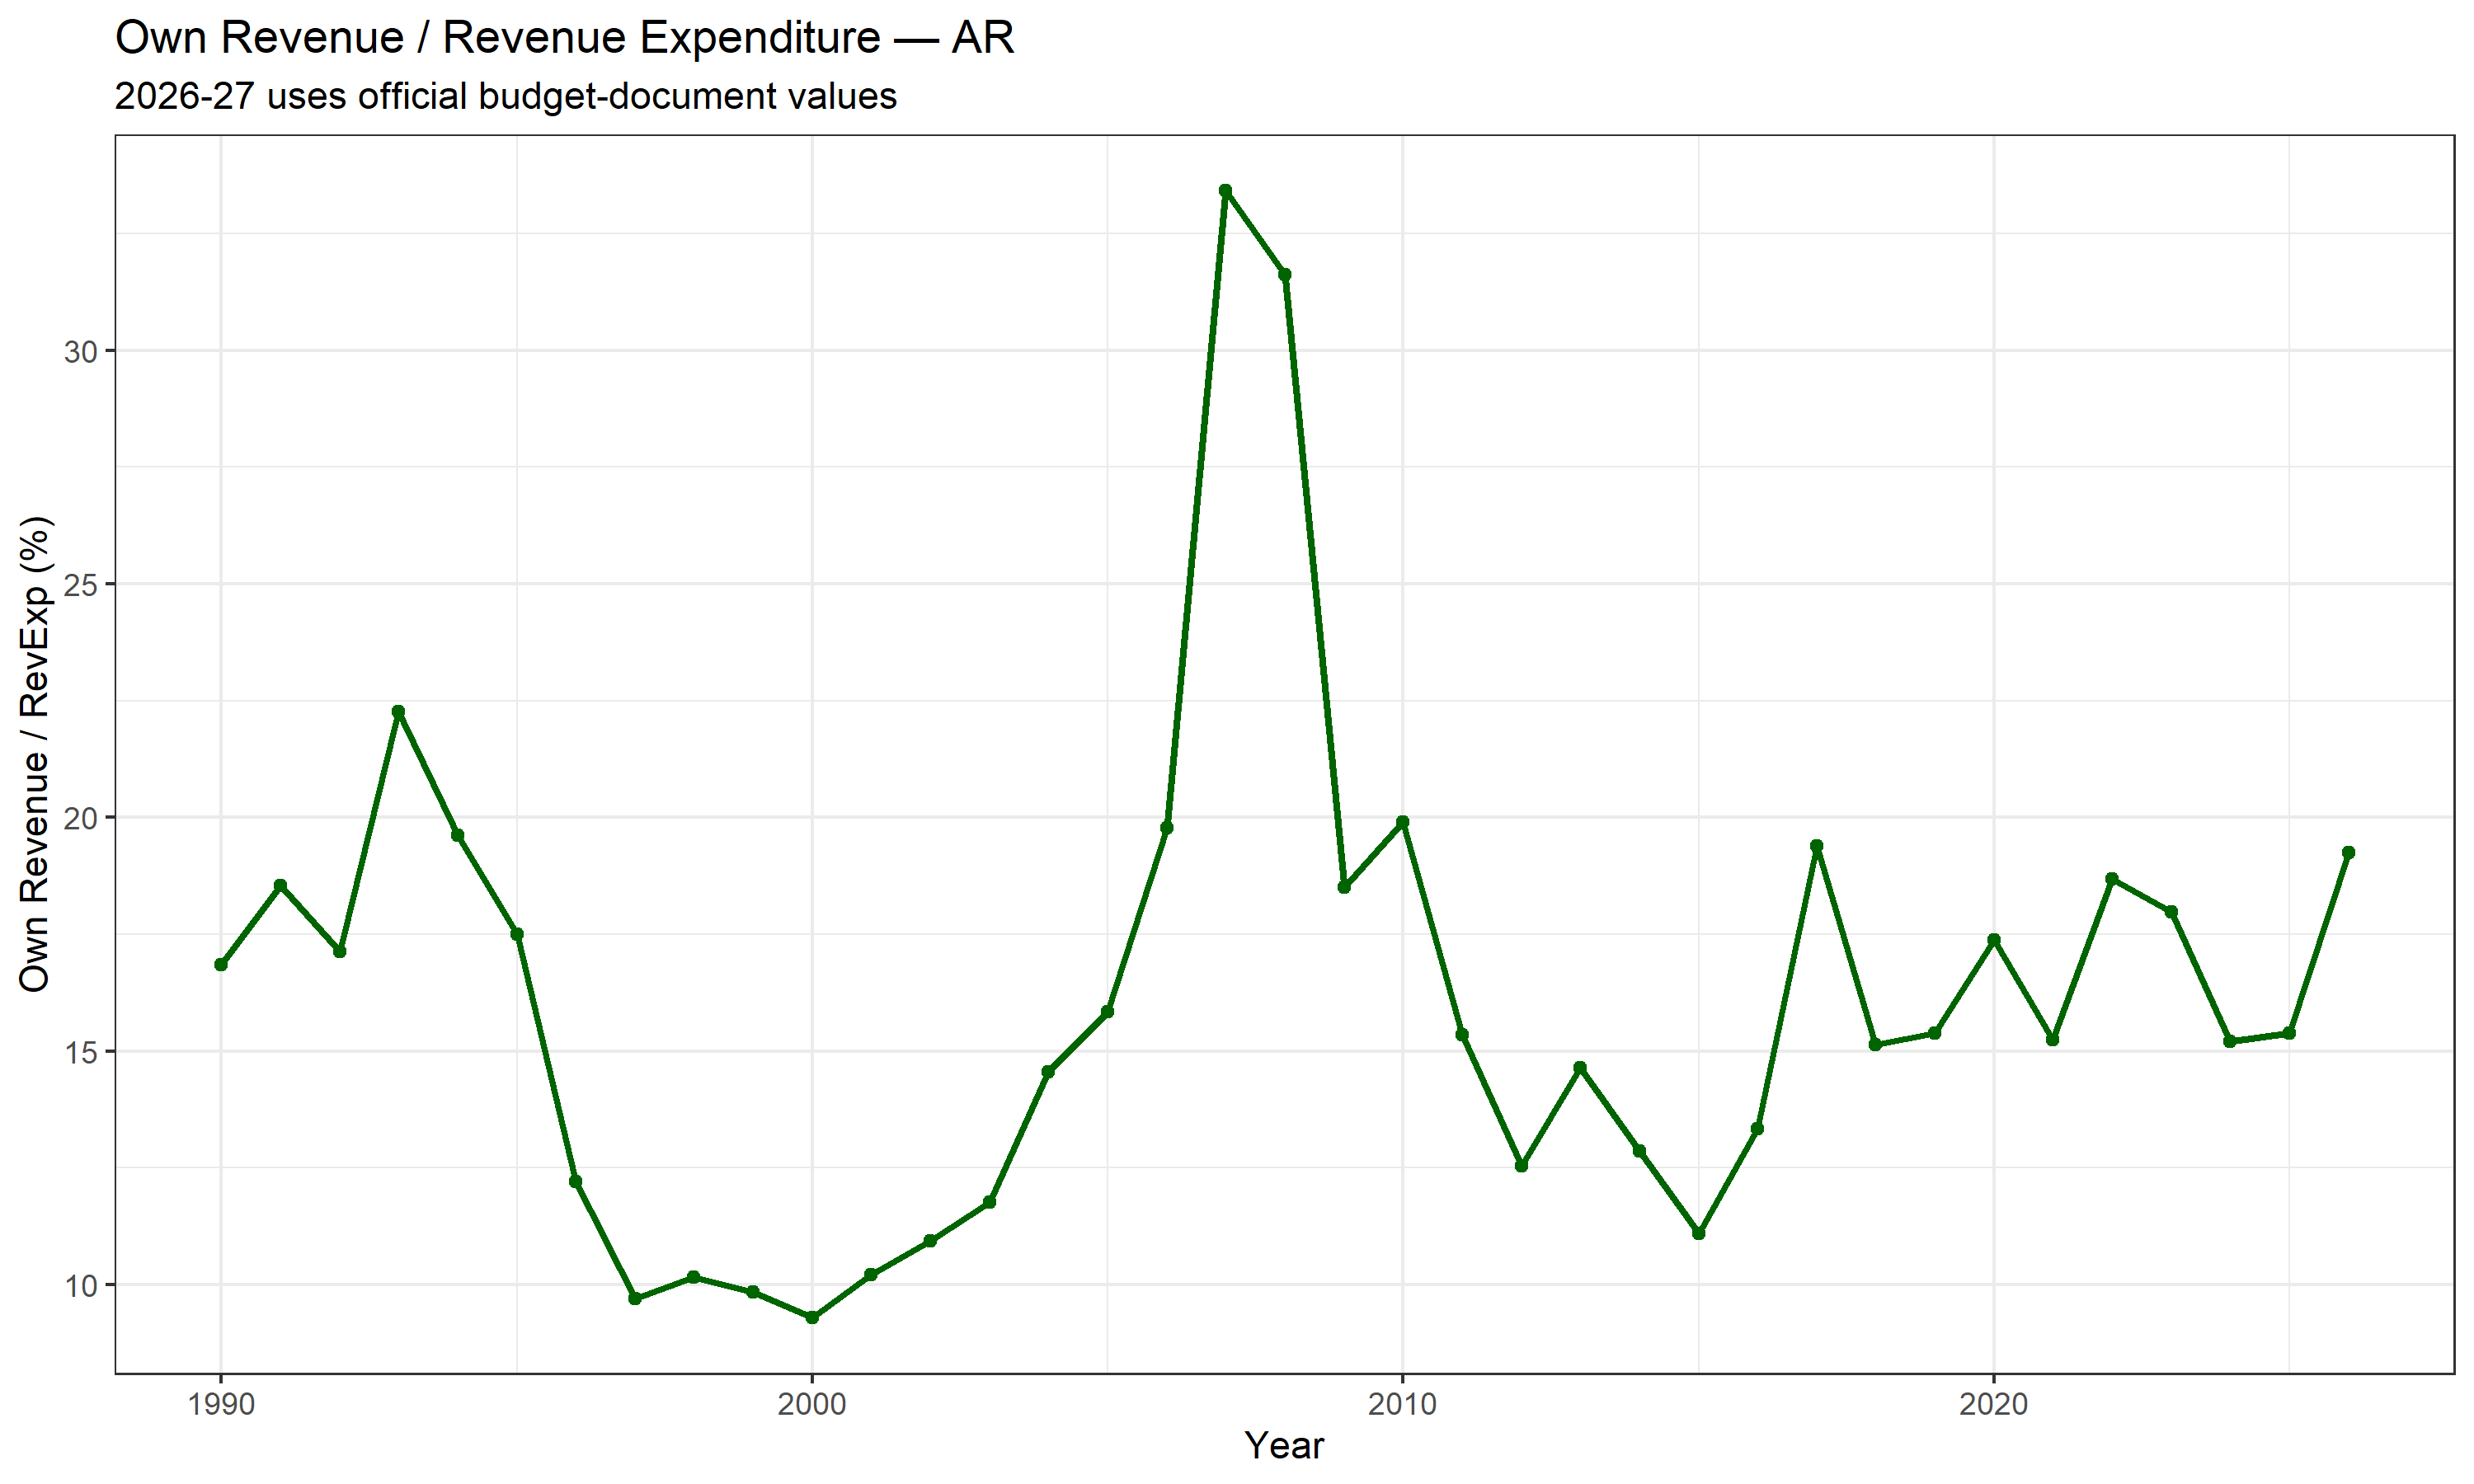
\includegraphics[width=0.82\textwidth]{fig11_own_revenue_ratio.png}
\caption{Own revenue relative to revenue expenditure}
\label{fig:ownrev}
\end{figure}

\begin{figure}[H]
\centering
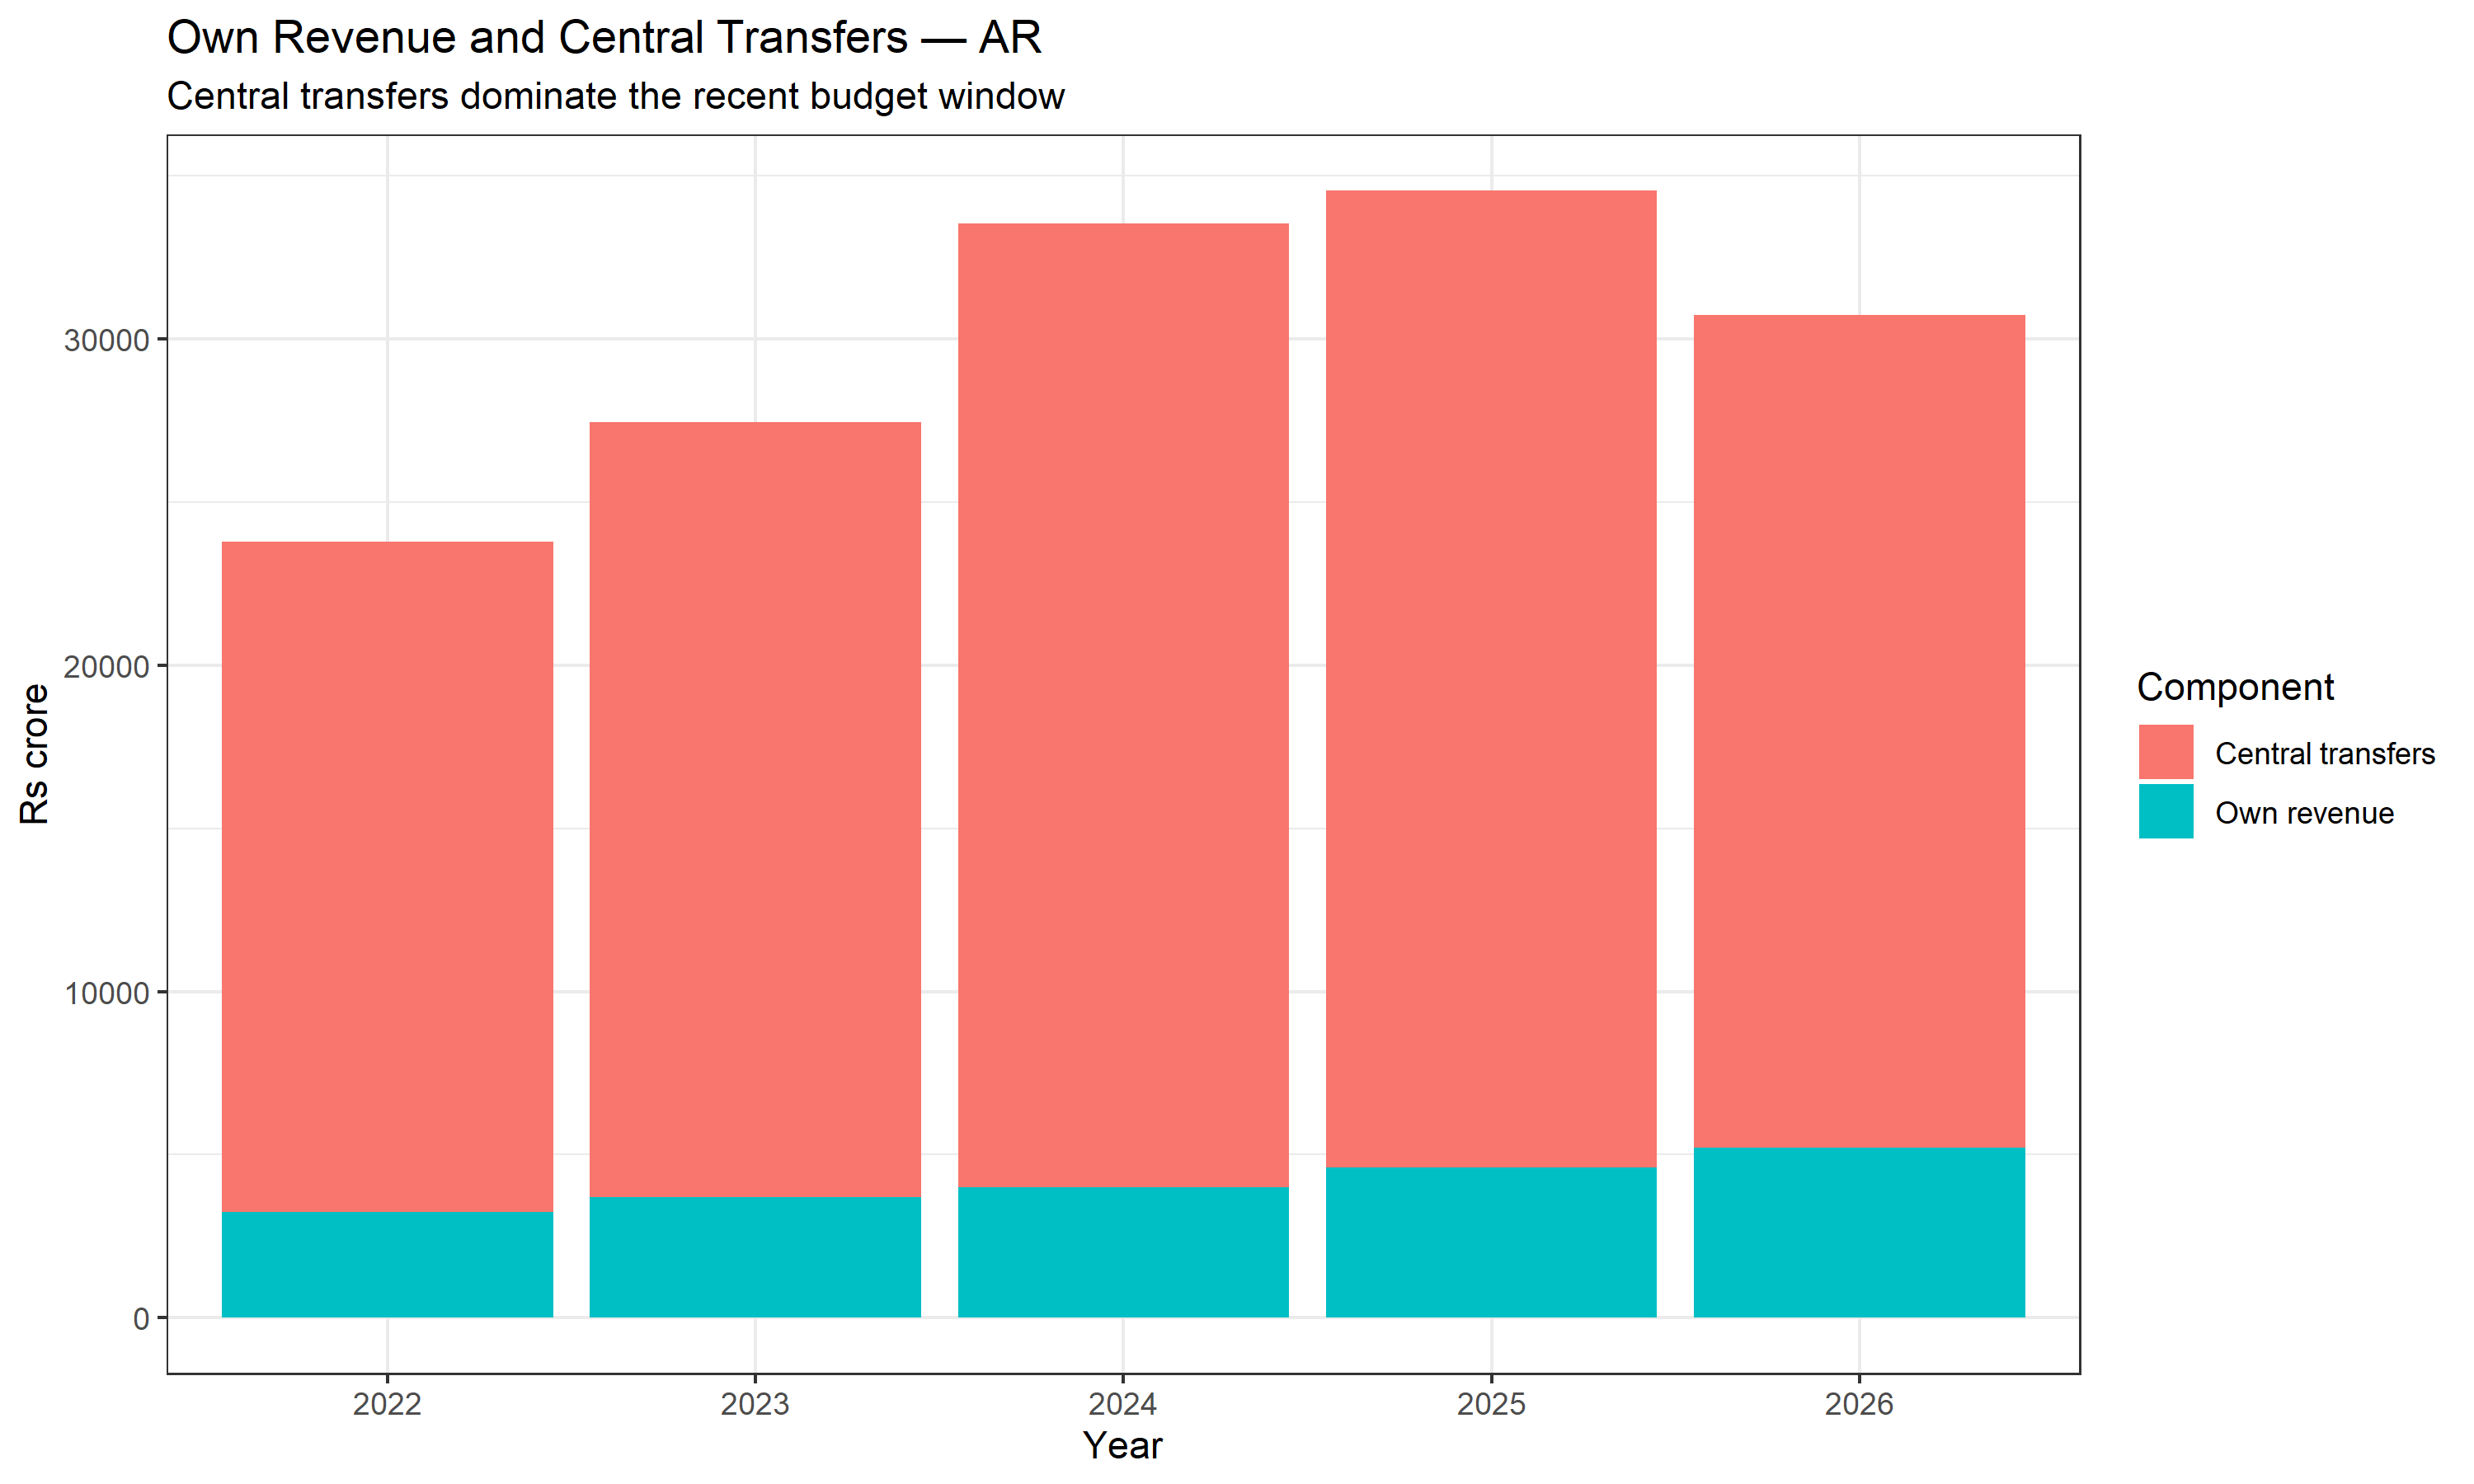
\includegraphics[width=0.82\textwidth]{fig18_project2_revenue_composition.png}
\caption{Own revenue versus central transfers in the recent budget window}
\label{fig:revmix}
\end{figure}

\subsection{Deficit reconciliation, central capex loans, and FRBM interpretation}

The most important methodological result of the paper is the gap between the broad PRS-style fiscal deficit and the official state-budget deficit. In 2025-26, the broad balance is about -10.5 percent of GSDP, but the official state-budget balance is only -1.6 percent of GSDP. In 2026-27, the broad balance is about -11.0 percent of GSDP, while the official balance is -1.7 percent. The difference is explained by the treatment of 50-year interest-free central capex loans.

The Annual Financial Statement records these loans on the capital-receipts side, under loans and advances from the Central Government. The PRS Budget Analysis reports them as ``central capex loans'' of Rs 3,704 crore in 2025-26 revised estimates and Rs 3,850 crore in 2026-27 budget estimates. The Arunachal FRBM statement then clarifies the operative fiscal-rule treatment: the normal net-borrowing limit is fixed at 3 percent of GSDP for 2026-27 to 2030-31, while Union on-lending under SASCI is over and above this limit. The same cash inflow therefore has two different meanings. In a broad resource-flow measure, it is borrowing that finances expenditure. In the official FRBM ceiling calculation, it is concessional capital support outside the ordinary borrowing limit.

This distinction matters for any discussion of FRBM compliance. If one reads only the official presentation, Arunachal Pradesh appears comfortably within a manageable fiscal range. If one reads the broader deficit concept, the state appears far more dependent on offsetting central support. Neither definition is simply wrong. They answer different questions. The official measure answers whether the state is inside the borrowing ceiling as currently interpreted. The broad measure answers how much of the spending programme is financed by receipts other than ordinary revenue. For sustainability analysis, the broad measure cannot be ignored, especially because the loans are large relative to GSDP even though they are interest-free and long maturity.

The sustainability implication is therefore nuanced. SASCI loans are not equivalent to market debt: they reduce interest pressure, support capital expenditure, and are intentionally designed to relax infrastructure constraints. But they also reveal that capital formation is being sustained by an exceptional central channel. If future Union support is reduced or if projects do not raise future economic and revenue capacity, the apparent FRBM comfort can coexist with a structural financing vulnerability.

\begin{figure}[H]
\centering
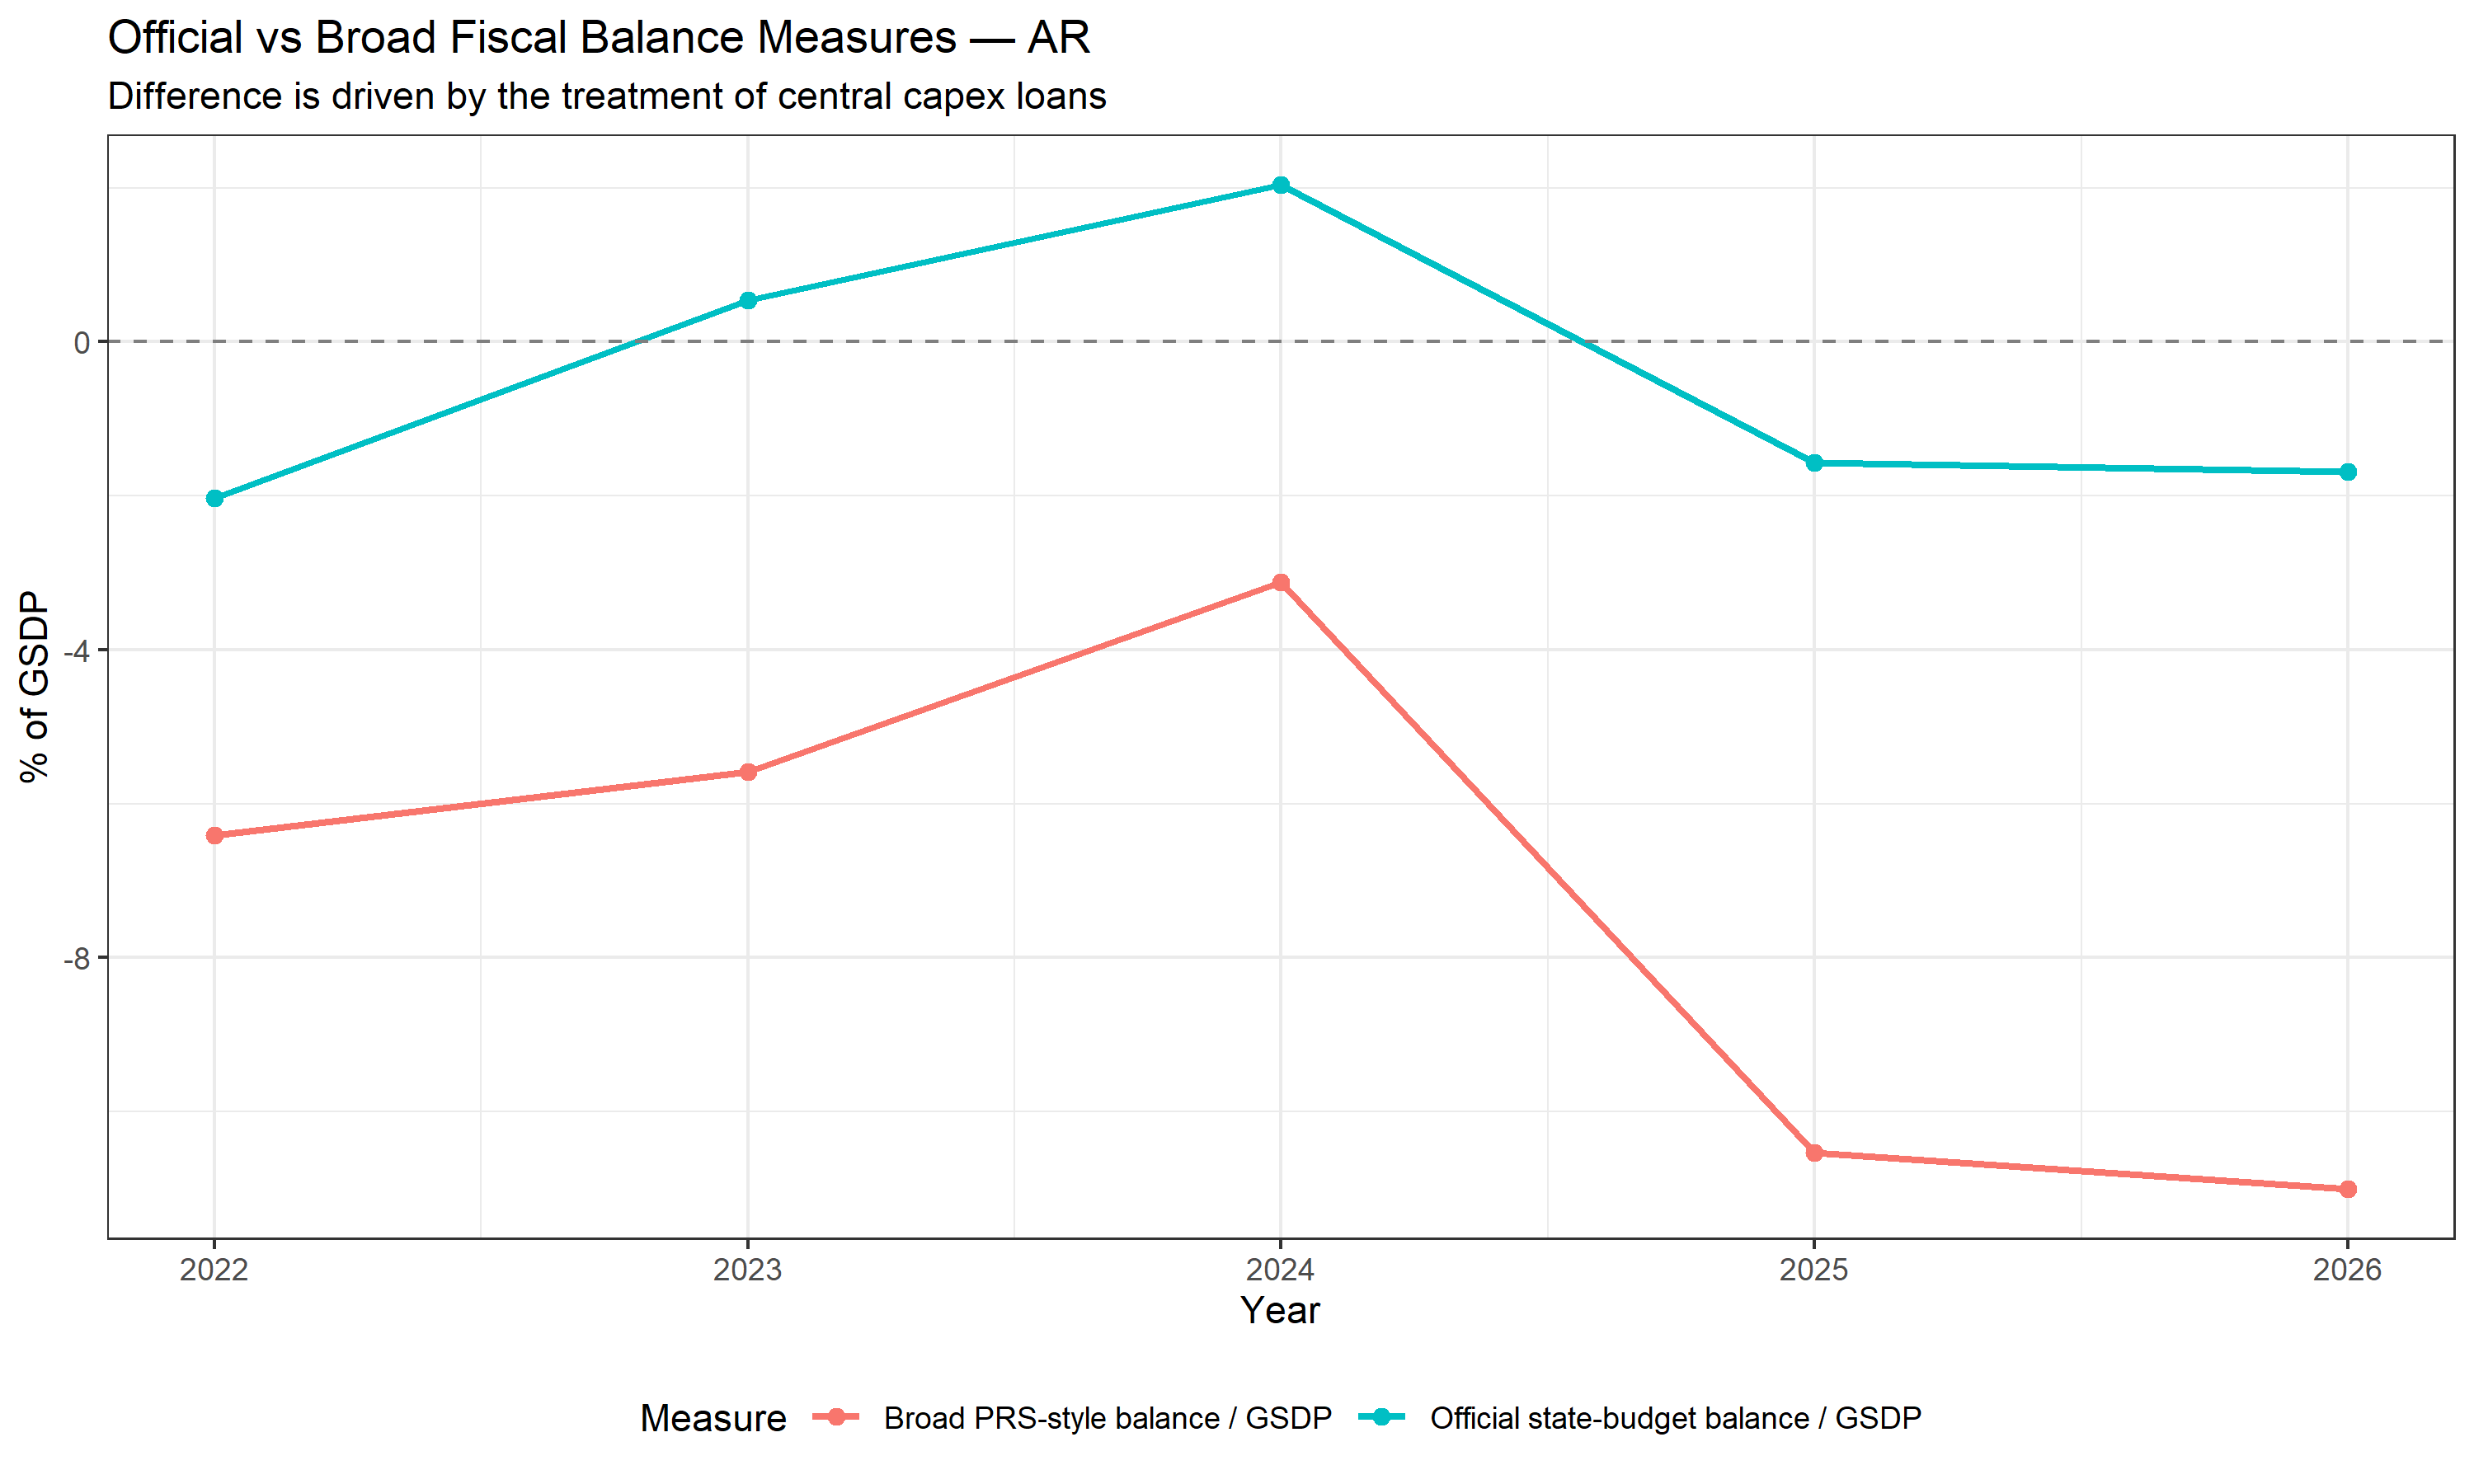
\includegraphics[width=0.82\textwidth]{fig17_project2_deficit_reconciliation.png}
\caption{Official versus broad fiscal balance measures}
\label{fig:recon}
\end{figure}

\subsection{Expenditure quality and committed burden}

Capital outlay remains substantial, but it is not sufficient on its own to prove deep structural transformation. In the five-year window, capital outlay ranges from 22 to 31 percent of total net expenditure. The state is therefore spending on asset creation, but that spending still operates inside a transfer-dependent structure.

The committed-expenditure trajectory also points in the same direction. PRS reports that committed expenditure was 34.3 percent of revenue receipts in 2024-25 actuals, 45.9 percent in 2025-26 revised estimates, and 60.2 percent in the 2026-27 budget. Salaries alone rise to 46.4 percent of revenue receipts in 2026-27, pensions to 10.5 percent, and interest to 3.3 percent. This reinforces the argument that the state's fiscal room is shaped not only by borrowing but by the structure of public administration and transfer-financed expenditure commitments. A comparable salary series is not exposed in the RBI historical table at the same granularity, so the figure uses the official PRS/AFS budget-document window rather than imputing older salaries.

\begin{figure}[H]
\centering
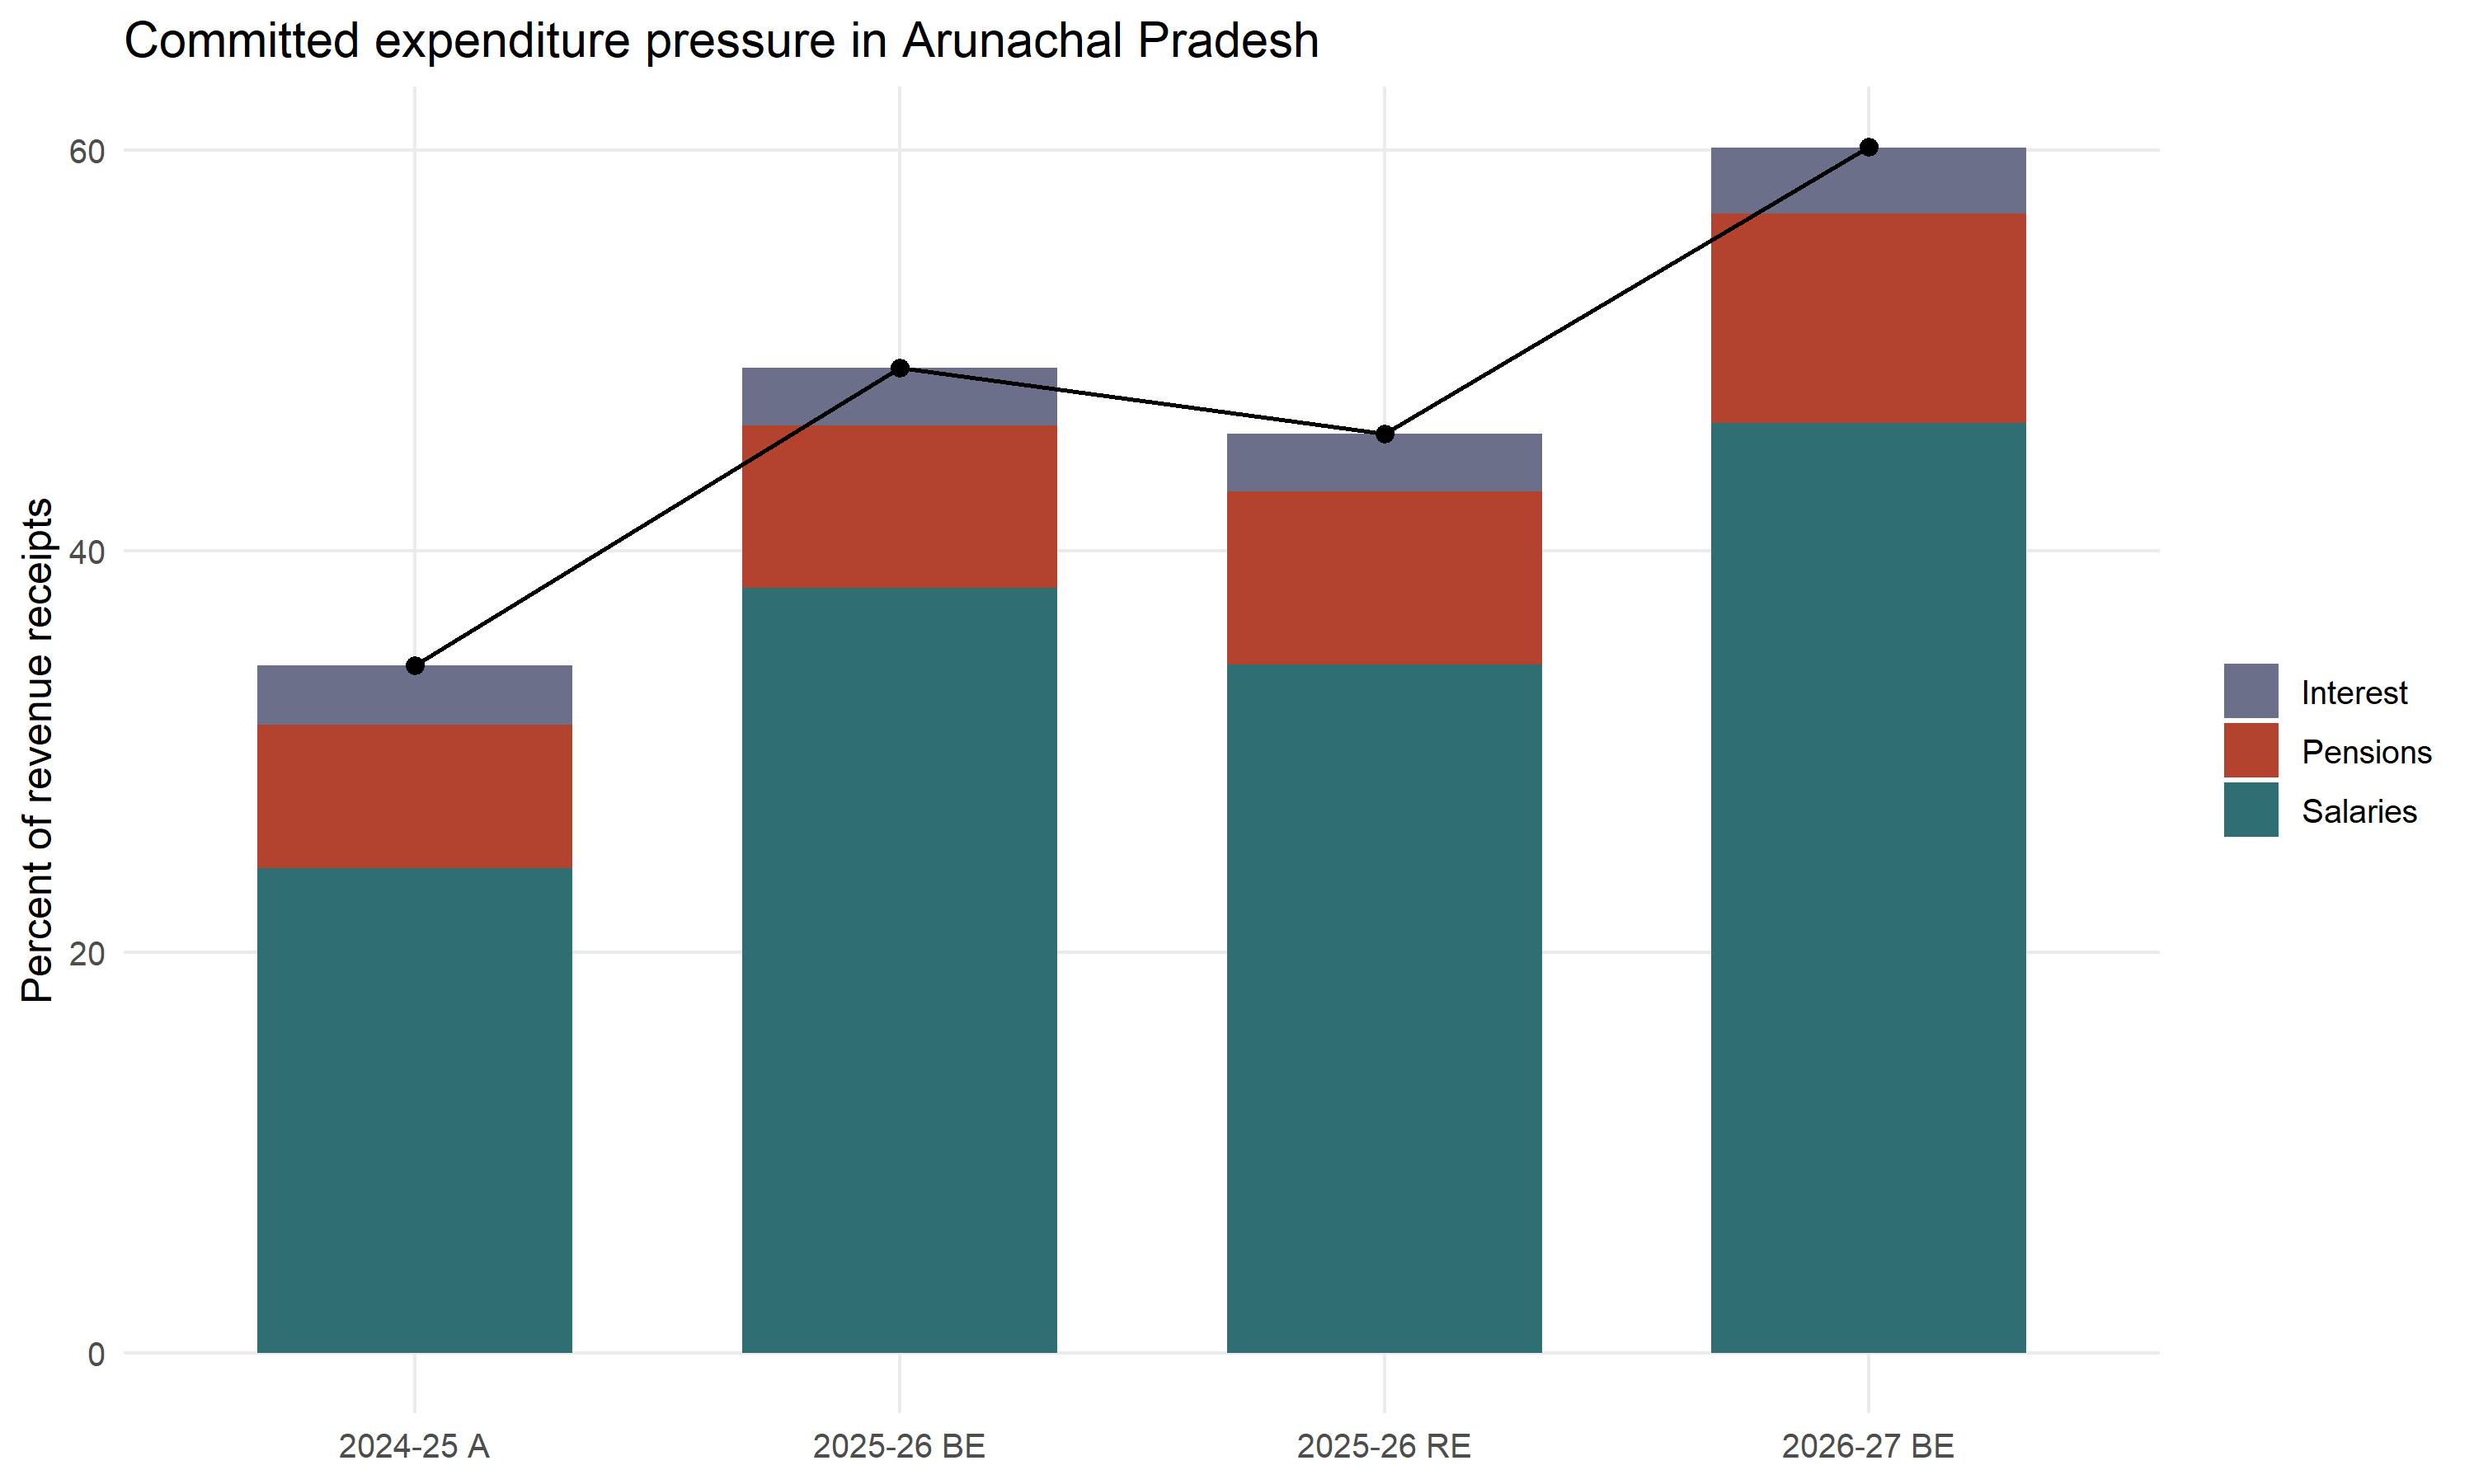
\includegraphics[width=0.86\textwidth]{fig23_project2_committed_expenditure_trajectory.png}
\caption{Committed expenditure pressure in Arunachal Pradesh}
\label{fig:committed}
\end{figure}

\subsection{Empirical Extension I --- Own Revenue Elasticity}

The first extension tests whether Arunachal Pradesh's own tax revenue responds to growth. The estimating equation is deliberately simple:
\[
\log(\text{Own Tax Revenue}_t)=\alpha+\beta \log(\text{GSDP}_t)+u_t .
\]
The sample uses account data from the RBI State Finance Database and current-price GSDP for 1990-91 to 2023-24. Standard errors are heteroskedasticity-robust using the HC1 correction.

\begin{table}[H]
\centering
\caption{Own-tax buoyancy regression, Arunachal Pradesh}
\small
\begin{tabular}{L{3.0cm}C{2.0cm}C{1.8cm}C{1.8cm}C{1.6cm}C{1.6cm}}
\toprule
Variable & Coefficient & HC1 s.e. & t-statistic & $N$ & $R^2$ \\
\midrule
$\log(\text{GSDP})$ & 1.694 & 0.032 & 52.13 & 34 & 0.988 \\
Intercept & -10.076 & 0.285 & -35.39 & 34 & 0.988 \\
\bottomrule
\end{tabular}
\caption*{\footnotesize Notes: Dependent variable is log own tax revenue. Sample is 1990-91 to 2023-24. P-values are below 0.001 under a normal approximation.}
\end{table}

The estimated elasticity is about 1.69. This means the evidence does not support a claim that own-tax revenue is unresponsive to GSDP. It is buoyant in percentage terms. However, the high $R^2$ is exactly why the regression needs time-series diagnostics. Two trending fiscal series can produce a misleadingly precise coefficient even when the relationship is not a valid long-run equilibrium.

\begin{table}[H]
\centering
\caption{Stationarity and cointegration diagnostics for the buoyancy regression}
\small
\begin{tabular}{L{4.1cm}C{2.1cm}C{1.7cm}C{1.7cm}L{3.4cm}}
\toprule
Series/test & Deterministic terms & Statistic & p-value & Inference \\
\midrule
ADF: log own tax revenue & constant + trend & -3.624 & 0.028 & Reject unit root at 5\% \\
ADF: log GSDP & constant + trend & -4.583 & 0.001 & Reject unit root at 5\% \\
ADF: OLS residual & none & -3.055 & 0.002 & Residual ADF rejects \\
Engle-Granger test & constant & -3.055 & 0.098 & Does not reject no cointegration at 5\% \\
\bottomrule
\end{tabular}
\caption*{\footnotesize Notes: ADF lag length is selected by AIC. The residual ADF p-value is reported as a diagnostic, while the Engle-Granger p-value is the more appropriate cointegration decision rule for the two-step regression.}
\end{table}

The diagnostics change the interpretation. The individual ADF tests with a deterministic trend reject unit roots in both log series, so the strongest spurious-regression concern is partly reduced. But the Engle-Granger test does not reject no cointegration at the 5 percent level; the p-value is about 0.098. The elasticity should therefore be read as a descriptive long-run association, not as a fully established cointegrating relationship. The paradox remains: the own-tax base starts from such a small level, and expenditure need is so transfer-financed, that even buoyant own-tax growth does not produce fiscal autonomy. This finding is consistent with the transfer literature's warning that own-revenue effort must be interpreted relative to expenditure responsibilities and transfer design, not only relative to state income \cite{bird_smart_2002,bhatt_scaramozzino_2015}.

\begin{figure}[H]
\centering
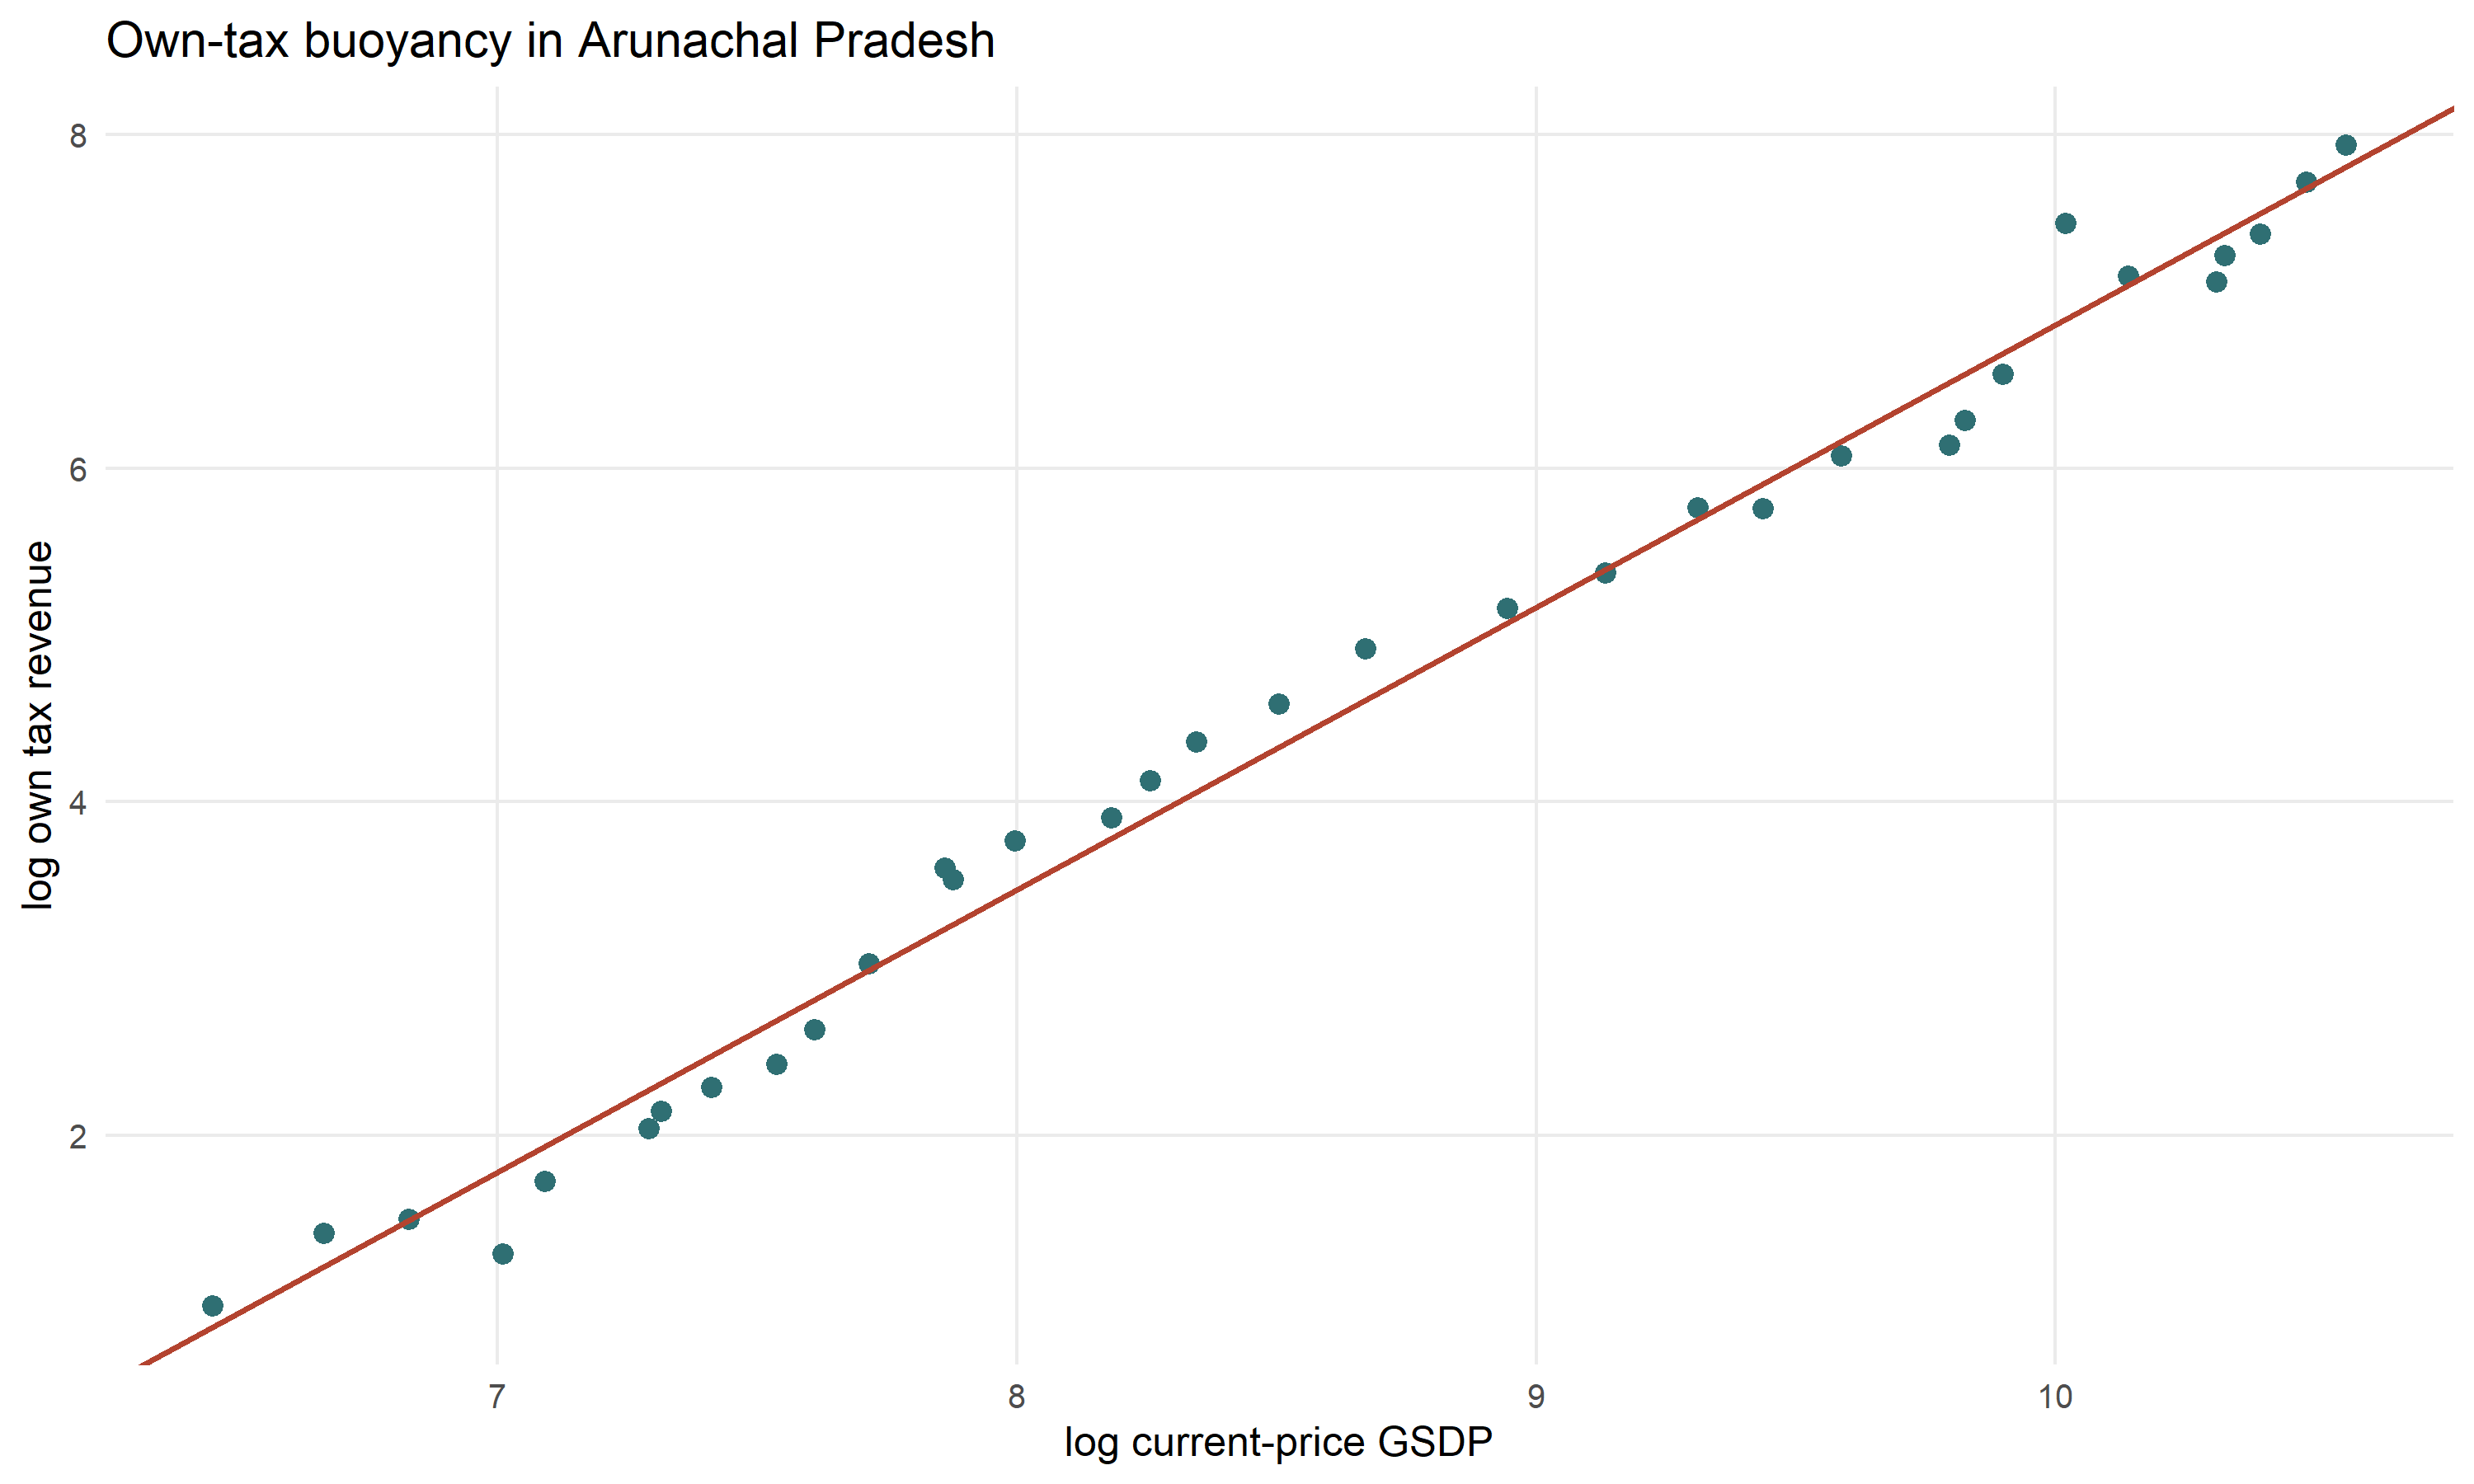
\includegraphics[width=0.82\textwidth]{fig19_project2_tax_buoyancy.png}
\caption{Own-tax buoyancy in Arunachal Pradesh}
\label{fig:taxbuoyancy}
\end{figure}

\subsection{Empirical Extension II --- Transfer Shock Simulation}

The second extension simulates the fiscal effect of the change in Arunachal Pradesh's devolution share from 1.76 under the 15th Finance Commission to 1.35 under the 16th Finance Commission. The 2026-27 budget is treated as the post-change case. A no-share-cut counterfactual is constructed by applying the old 1.76 share to the same implied divisible pool. This is not a forecast of all transfers; it isolates the mechanical devolution-share effect.

\begin{table}[H]
\centering
\caption{16th Finance Commission devolution-share simulation, 2026-27}
\scriptsize
\setlength{\tabcolsep}{3pt}
\begin{tabular}{L{4.2cm}C{1.2cm}C{1.8cm}C{1.8cm}C{1.9cm}C{1.8cm}}
\toprule
Scenario & Share & Tax devol. & Revenue balance & Official fiscal deficit & Broad fiscal deficit \\
\midrule
15th FC share retained & 1.760 & 26,941 & 9,948 & -5,577 & -1,727 \\
Half of share-loss shock & 1.555 & 23,803 & 6,810 & -2,439 & 1,411 \\
Full 16th FC share-loss shock & 1.350 & 20,665 & 3,672 & 699 & 4,549 \\
Stress: 125 percent shock & 1.248 & 19,096 & 2,103 & 2,268 & 6,118 \\
\bottomrule
\end{tabular}
\caption*{\footnotesize Notes: Amounts are Rs crore. Negative deficit values denote surplus. The full 16th FC shock is the 2026-27 budget case.}
\end{table}

The simulation shows why the revenue surplus is fragile. If the old devolution share had been retained on the same implied divisible pool, the 2026-27 revenue balance would have been about Rs 9,948 crore. Under the 16th FC share, it is Rs 3,672 crore. The state remains in revenue surplus, but the margin is reduced by roughly Rs 6,276 crore. Under the official deficit definition, the same shock moves the state from a large counterfactual surplus to a deficit of about Rs 699 crore. This is the revenue-surplus paradox in dynamic form: the surplus is not only transfer-dependent in levels; it is highly sensitive to the rules governing transfers \cite{rao_singh_2005,rangarajan_srivastava_2011}.

\begin{figure}[H]
\centering
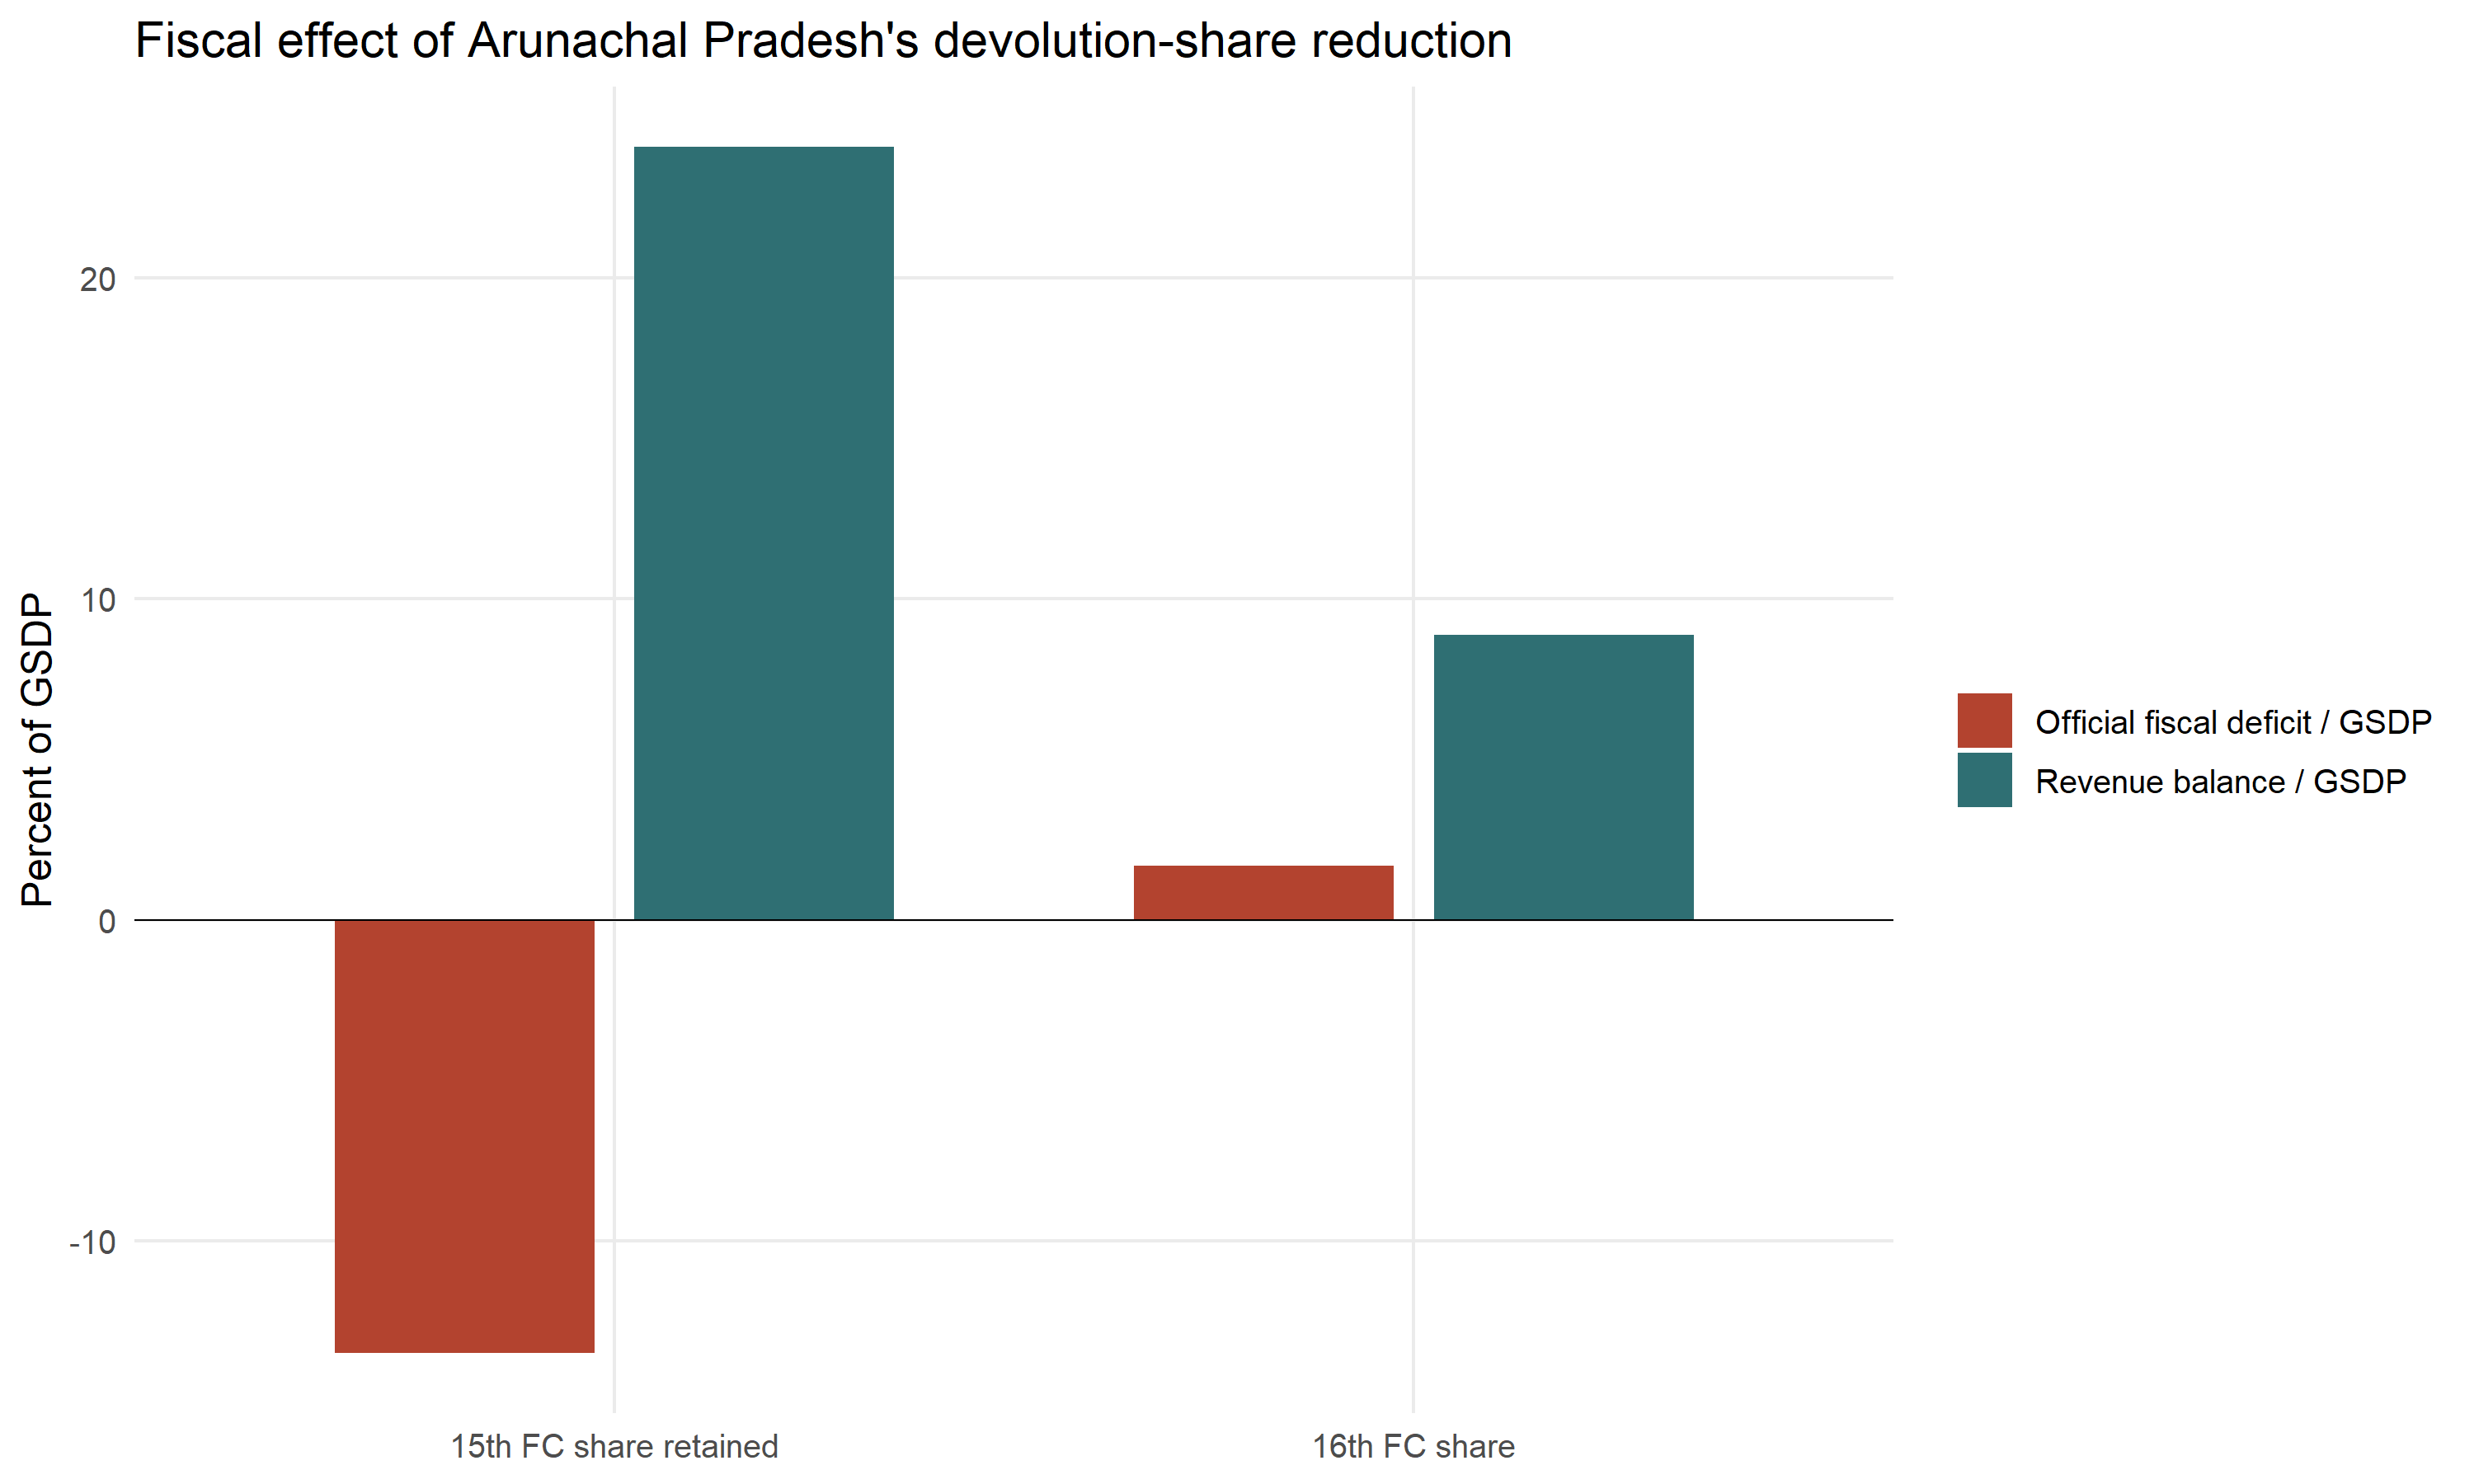
\includegraphics[width=0.82\textwidth]{fig20_project2_transfer_shock.png}
\caption{Fiscal effect of the devolution-share reduction}
\label{fig:transferstress}
\end{figure}

The 16th Finance Commission simulation can be extended from a one-year counterfactual into a 2026-31 transfer path. The Commission's local-body and disaster-management grants for Arunachal Pradesh add up to Rs 2,548 crore over the award period: Rs 1,698 crore for rural local bodies, Rs 233 crore for urban local bodies, and Rs 616 crore for disaster management \cite{prs16fc}. Because the year-wise grant release path is not specified in the PRS summary, Table \ref{tab:fcpath} distributes these grants evenly and applies an illustrative 8 percent nominal growth path to tax devolution and revenue expenditure, holding non-Finance-Commission grants at the 2026-27 level. This is not a forecast. It is a transparent sensitivity path showing how much surplus remains under the new transfer regime.

\begin{table}[H]
\centering
\caption{Illustrative 16th Finance Commission transfer trajectory, 2026-31}
\label{tab:fcpath}
\small
\begin{tabular}{L{1.8cm}C{2.2cm}C{2.1cm}C{2.2cm}C{2.0cm}}
\toprule
Year & Tax devolution & FC local/disaster grants & Revenue balance & Revenue balance / GSDP \\
\midrule
2026-27 & 20,665 & 510 & 3,821 & 9.25 \\
2027-28 & 22,318 & 510 & 3,726 & 8.35 \\
2028-29 & 24,104 & 510 & 3,623 & 7.52 \\
2029-30 & 26,032 & 510 & 3,512 & 6.75 \\
2030-31 & 28,115 & 510 & 3,392 & 6.04 \\
\bottomrule
\end{tabular}
\caption*{\footnotesize Notes: Amounts are Rs crore except the final column. The path assumes 8 percent nominal growth in devolution, own revenue, revenue expenditure, and GSDP; non-FC grants are held at their 2026-27 level.}
\end{table}

\begin{figure}[H]
\centering
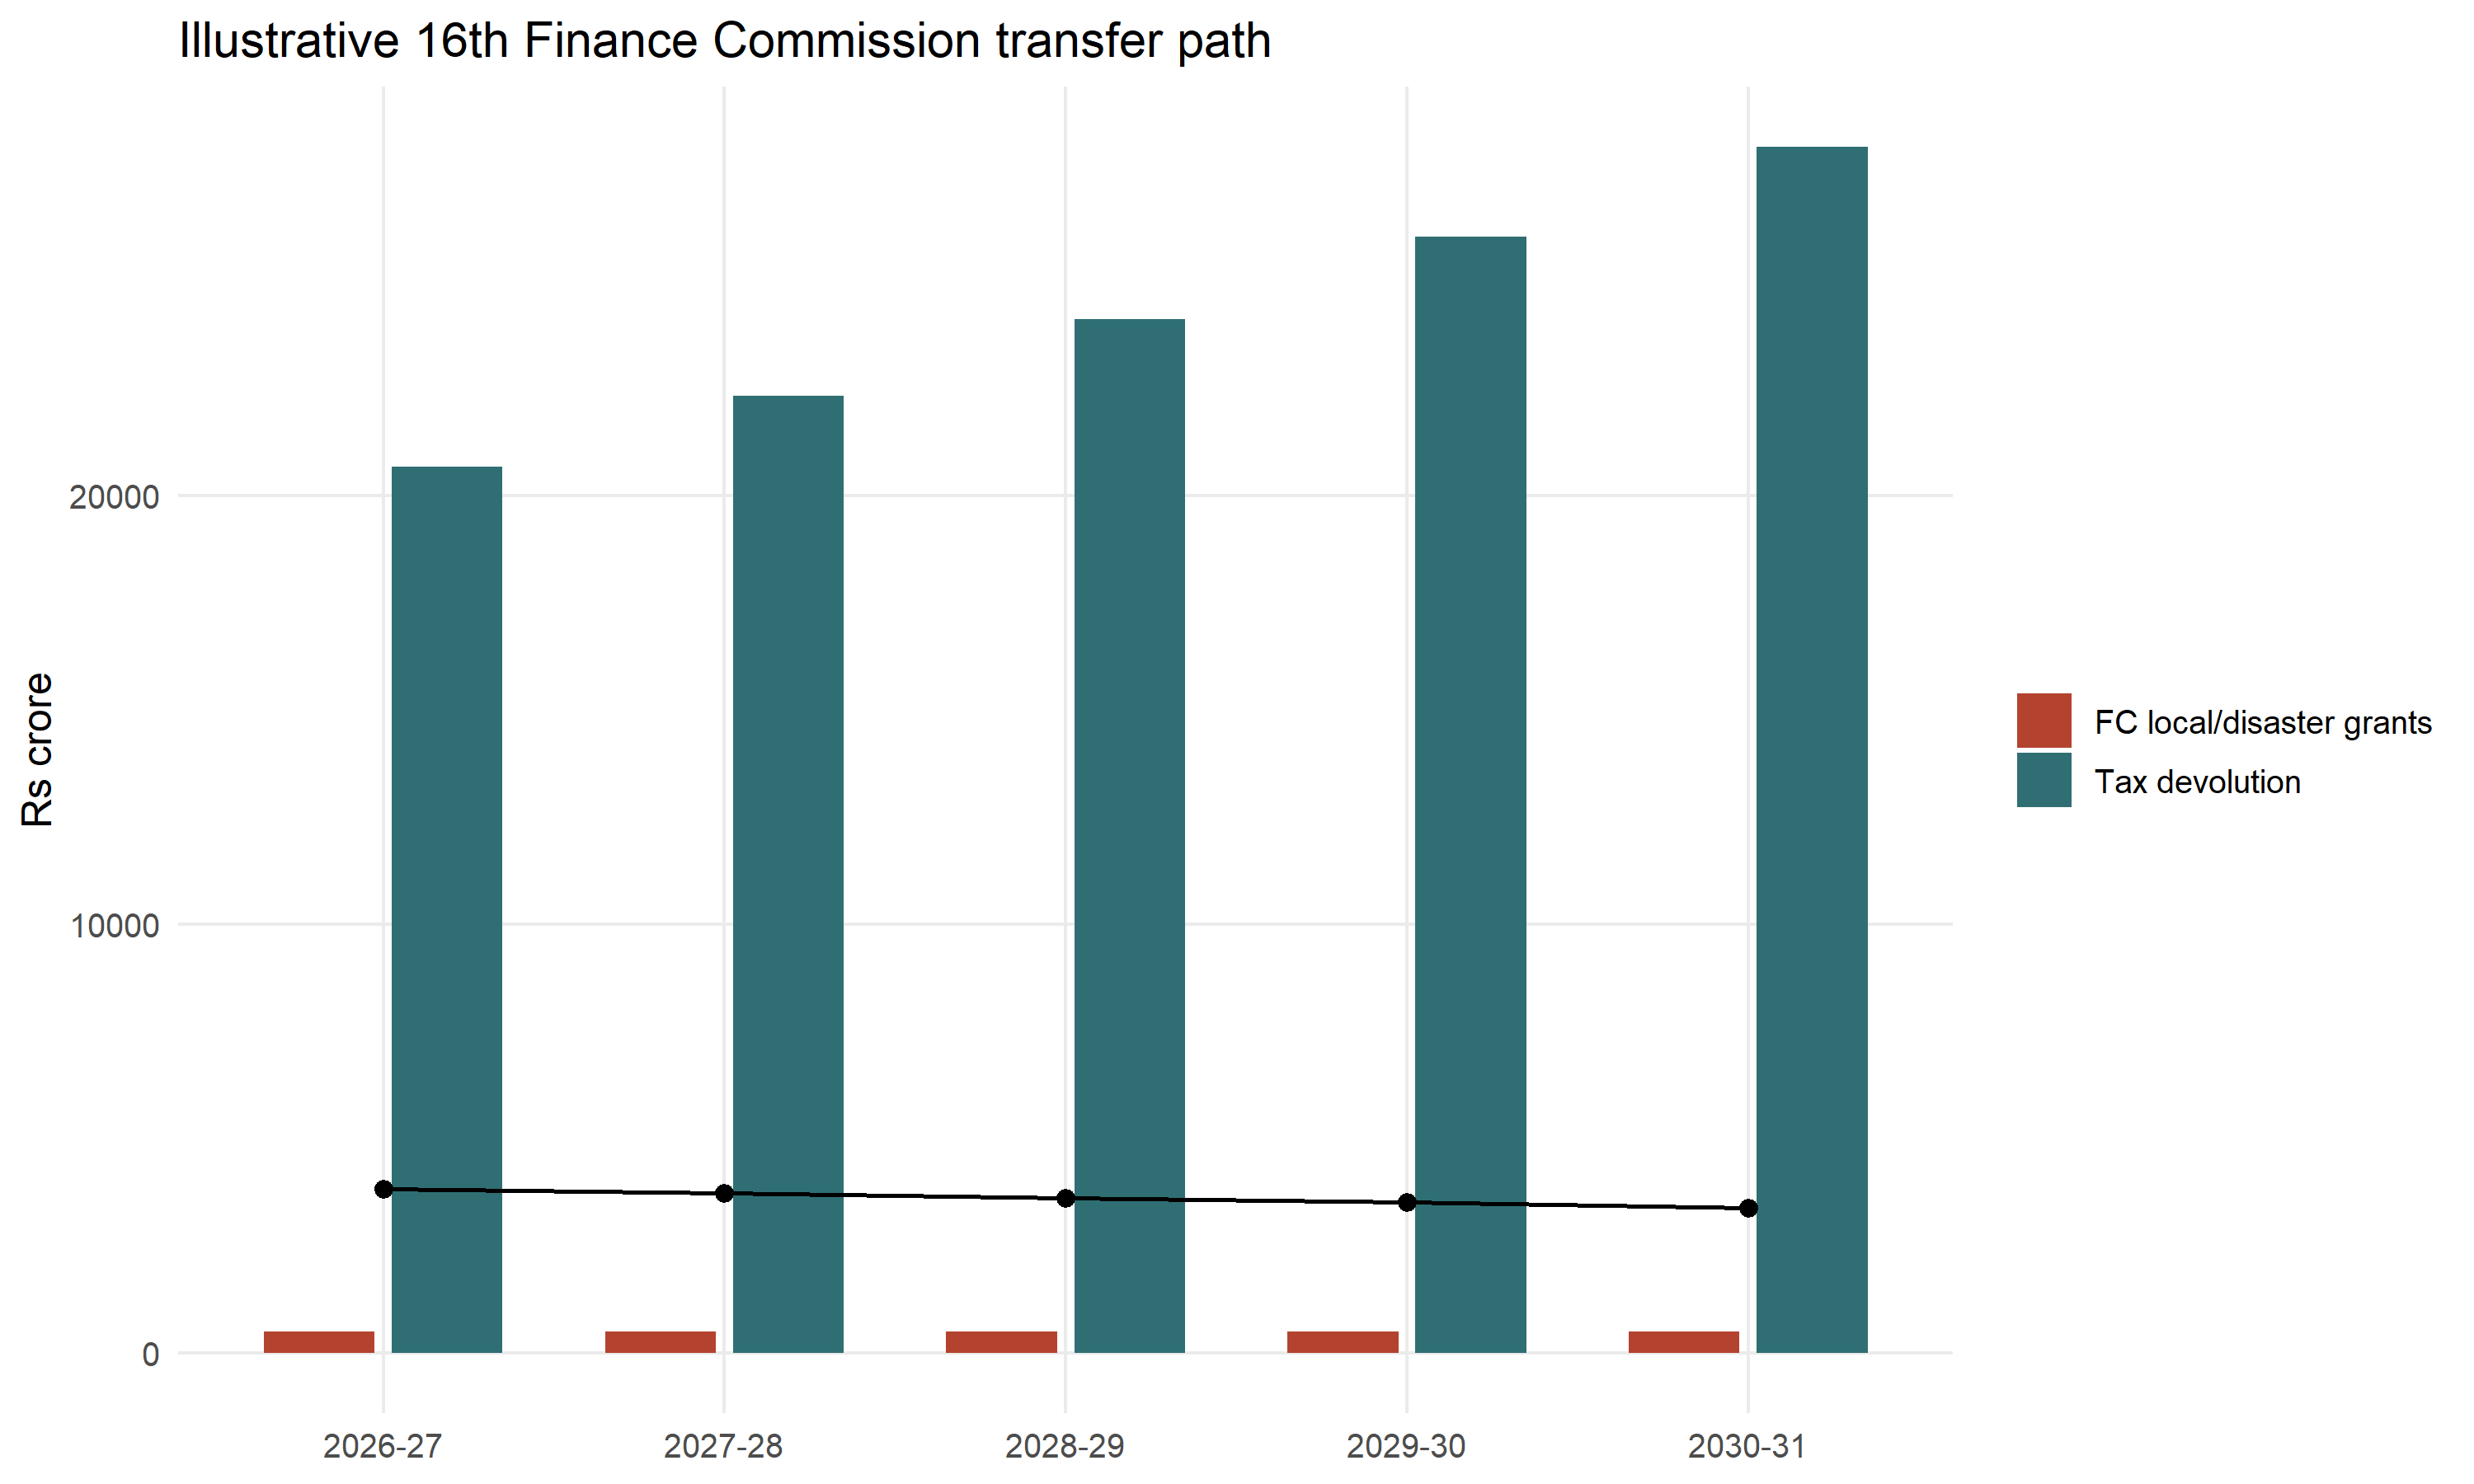
\includegraphics[width=0.84\textwidth]{fig25_project2_16fc_transfer_trajectory.png}
\caption{Illustrative 16th Finance Commission transfer path}
\label{fig:fcpath}
\end{figure}

The extended path shows that the revenue balance remains positive under the mechanical scenario, but the surplus ratio falls from 9.25 percent of GSDP in 2026-27 to 6.04 percent by 2030-31. The reason is that the state loses the old 1.76 percent devolution share and receives relatively small formula grants in comparison with tax devolution. This strengthens the main argument: the critical issue is not whether Arunachal Pradesh is immediately at risk of revenue deficit, but whether a transfer-dependent surplus can be converted into greater own-source capacity before the next transfer shock.

\subsection{Empirical Extension III --- Cross-State Evidence}

The third extension asks whether Arunachal Pradesh is unique or part of a broader frontier-state pattern. The comparison uses 2023-24 account figures from the all-state RBI database for Arunachal Pradesh, Assam, Sikkim, Himachal Pradesh, Tripura, and Meghalaya. This account-year comparison avoids mixing actuals with revised or budget estimates.

\begin{table}[H]
\centering
\caption{Cross-state fiscal comparison, 2023-24 accounts}
\small
\begin{tabular}{L{2.8cm}C{1.6cm}C{2.0cm}C{2.0cm}C{1.9cm}}
\toprule
State & Fiscal dependence & Own rev. / rev. exp. & Revenue balance / GSDP & Capital outlay ratio \\
\midrule
Arunachal Pradesh & 86.5 & 18.0 & 17.8 & 28.6 \\
Tripura & 83.8 & 18.2 & 2.8 & 12.4 \\
Meghalaya & 79.2 & 22.6 & 2.6 & 19.3 \\
Sikkim & 68.6 & 31.9 & 0.3 & 23.8 \\
Assam & 62.8 & 36.2 & -0.5 & 17.9 \\
Himachal Pradesh & 62.1 & 33.2 & -2.6 & 10.4 \\
\bottomrule
\end{tabular}
\caption*{\footnotesize Notes: Fiscal dependence is central taxes plus grants divided by total revenue receipts. Capital outlay ratio is capital outlay divided by revenue expenditure plus net capital expenditure.}
\end{table}

The comparison shows that Arunachal Pradesh is not simply an outlier because it is small. Tripura and Meghalaya also show high transfer dependence, but Arunachal Pradesh combines the highest dependence ratio with the largest revenue balance and the highest capital outlay ratio in the comparator group. Assam and Himachal Pradesh have much stronger own-revenue coverage, while Sikkim sits between the two groups. The pattern is therefore best described as a frontier-state gradient: Northeast and Himalayan states share transfer dependence, but Arunachal Pradesh is the clearest case of headline fiscal strength combined with weak fiscal autonomy.

\begin{figure}[H]
\centering
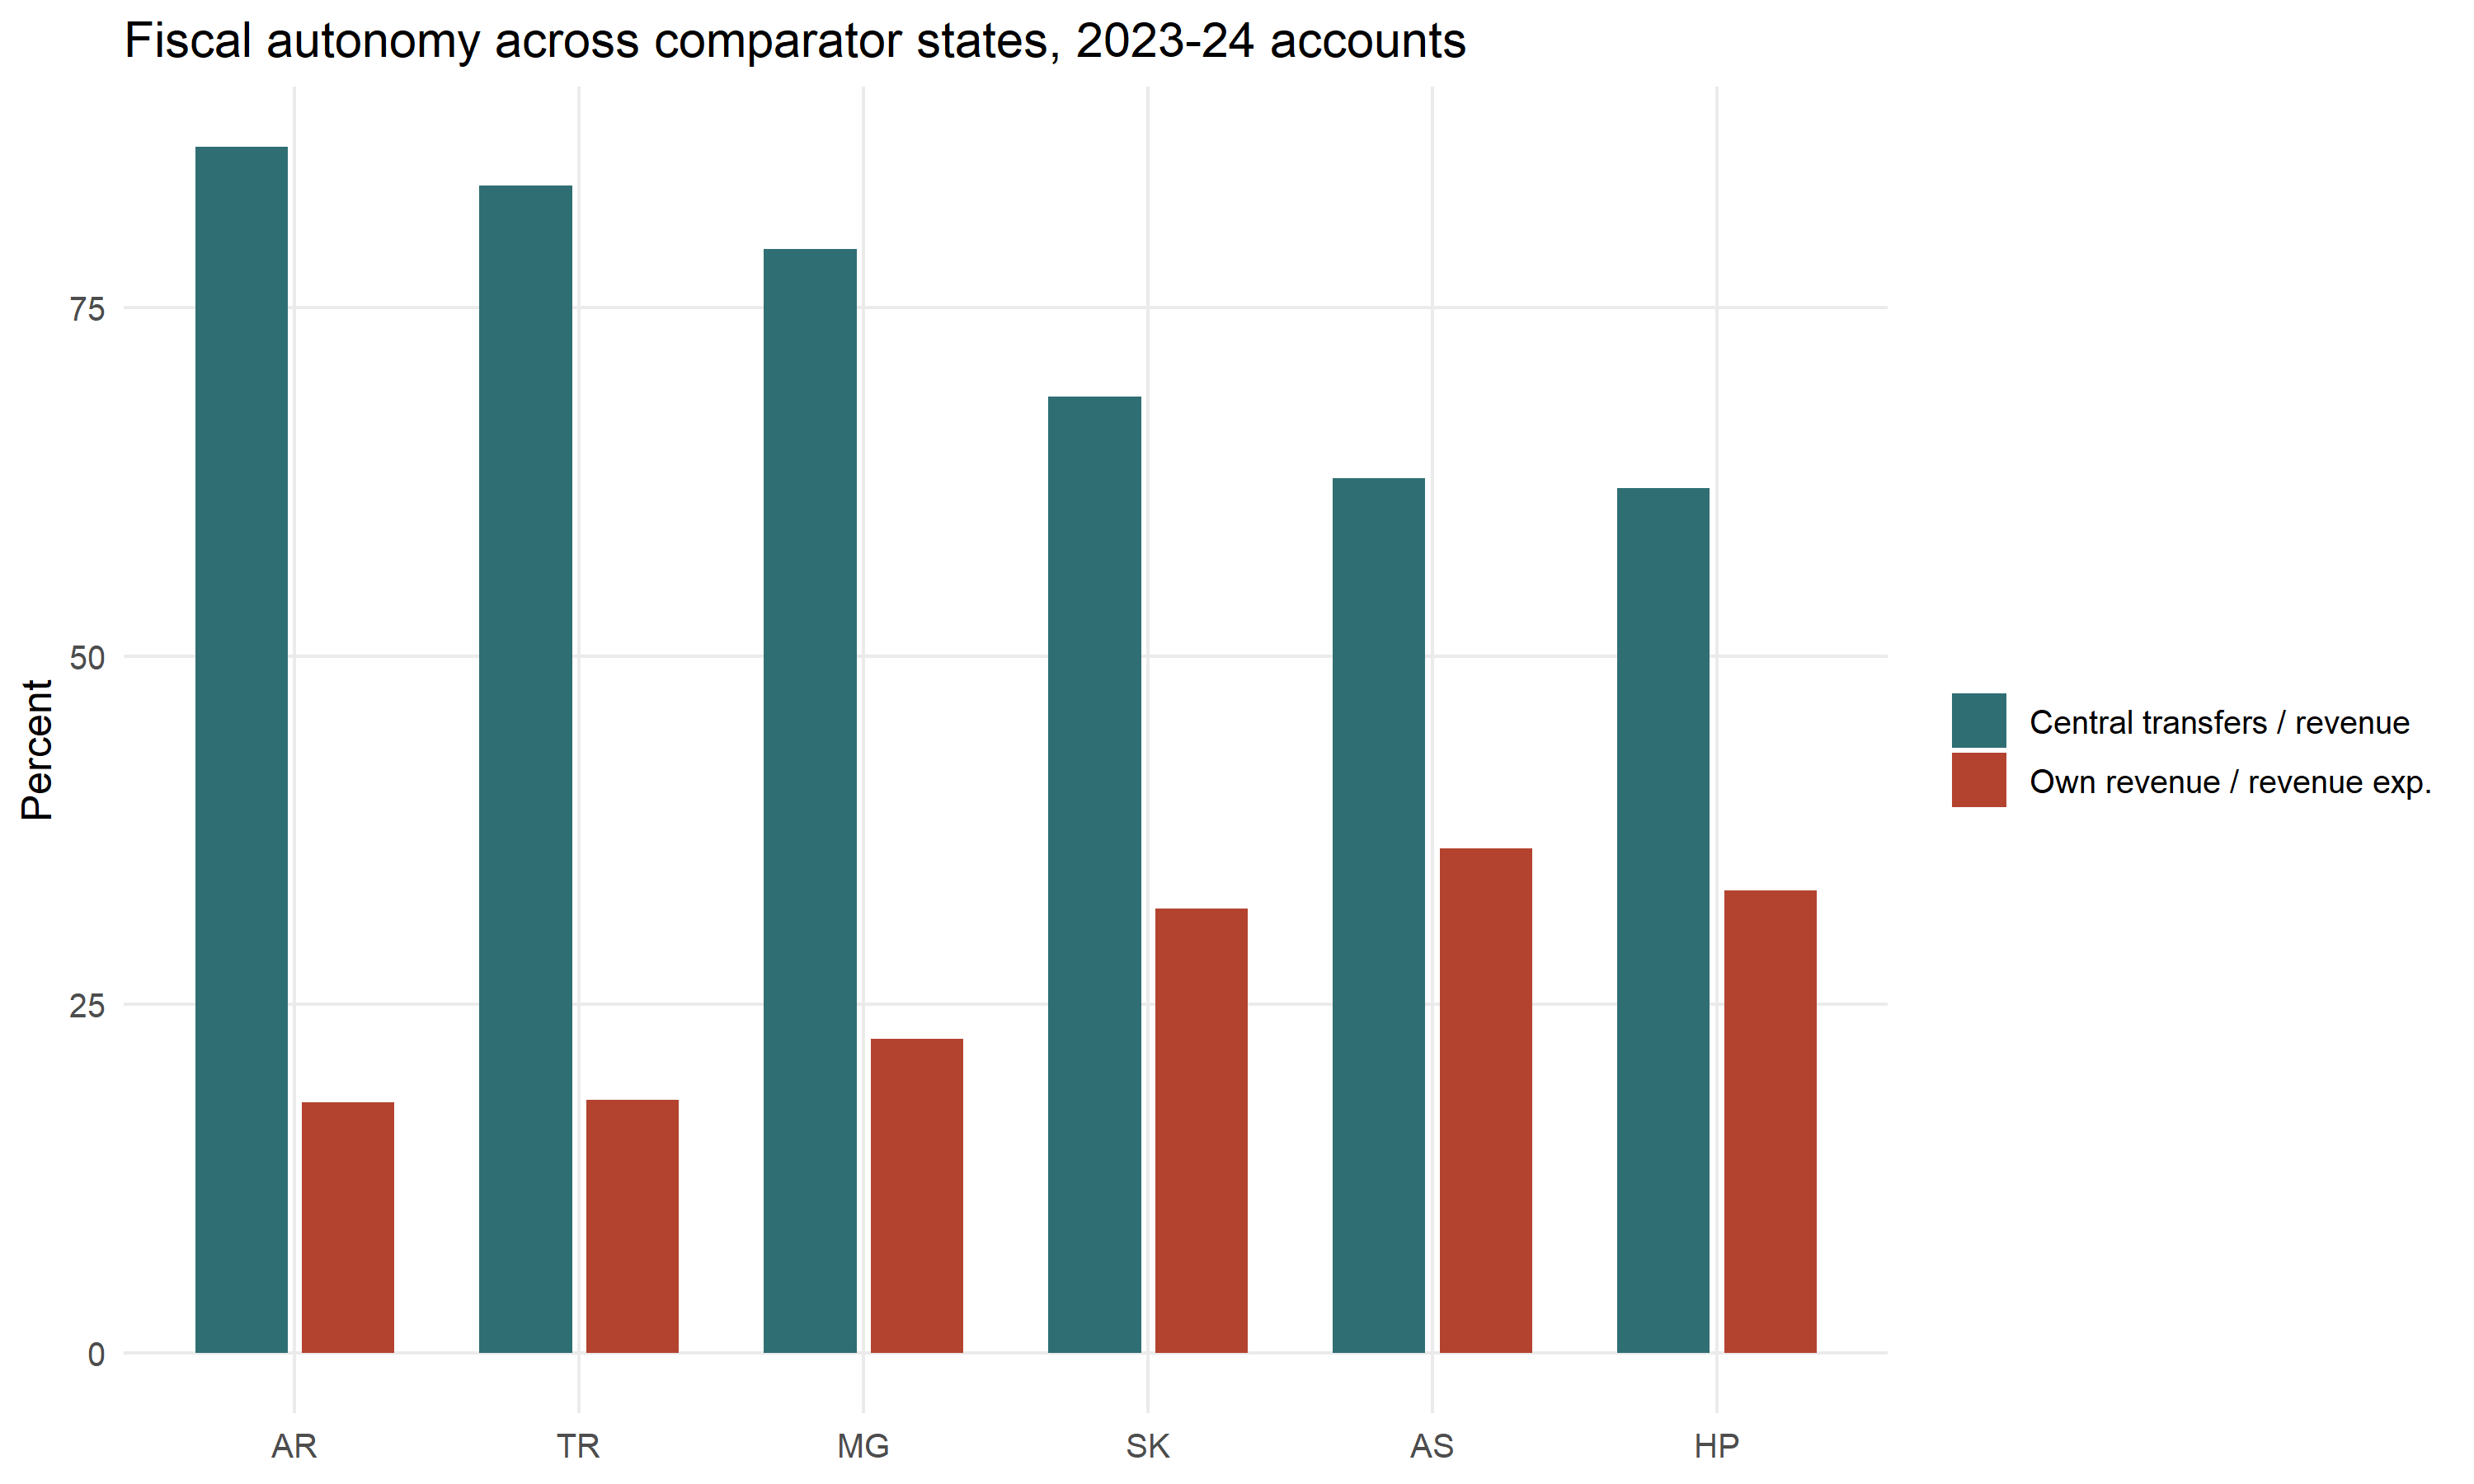
\includegraphics[width=0.82\textwidth]{fig21_project2_cross_state_comparison.png}
\caption{Fiscal autonomy across comparator states}
\label{fig:crossstate}
\end{figure}

\section{Linking Fiscal Health to the State's Growth Pattern}

Arunachal Pradesh's growth is real but not transformation-led in the classical industrialisation sense. Historical state-income analysis shows major growth shifts around 1995-96 and 2013-14, while the sectoral pattern is dominated by services and public administration rather than manufacturing. The fiscal evidence provides the counterpart to that growth pattern.

The common thread is that growth and fiscal strength are both supported by transfers and public expenditure rather than by a broad, self-sustaining productive base. This does not make the growth ``fake'' or the fiscal balances ``wrong''. It changes their interpretation. Arunachal Pradesh is best understood as a frontier economy in which the state apparatus and the transfer system play a constitutive role in both output expansion and fiscal stability.

\section{Policy Discussion}

The 16th Finance Commission context sharpens the policy relevance of the findings. PRS reports that Arunachal Pradesh's share in devolution falls from 1.76 under the 15th Finance Commission to 1.35 under the 16th. The simulation above shows that this change reduces the 2026-27 revenue surplus by about Rs 6,276 crore relative to a no-share-cut counterfactual. If the reduction is not offset by grants, own-resource mobilisation, or higher GSDP growth, the state's current fiscal structure becomes more fragile. The paper's argument is therefore forward-looking: today's strong revenue balance does not automatically translate into tomorrow's resilience.

The policy challenge is not to eliminate transfers in a strategically important frontier state. That would be unrealistic and undesirable. The challenge is to convert transfer-supported stability into a stronger own-revenue base and a more diversified economic structure. Four policy directions follow.

First, the state needs a practical own-tax strategy rather than a generic call for higher taxes. The buoyancy regression suggests that own tax revenue rises with GSDP, but the level remains too small. The immediate revenue base is concentrated in State GST, VAT/sales tax, excise, motor vehicles, stamps and registration, and land revenue. The highest-potential reforms are administrative: GST compliance analytics, better matching of e-way bills and registrations, stronger enforcement in border and construction supply chains, digitised vehicle and permit fees, and improved stamp-duty valuation in urbanising corridors such as Itanagar and the larger district headquarters. These measures are more credible than large new tax handles.

Second, non-tax revenue should be treated as a development-finance instrument. Arunachal Pradesh has hydro-power potential, forest and eco-tourism assets, minerals in limited areas, and user-charge possibilities in power, water, transport, and urban services. The point is not to impose high charges on poor households. It is to improve cost recovery where public services support commercial users and where leakage is high. The Rajiv Gandhi University evaluation already emphasised own non-tax revenue weakness and hydro-power potential \cite{nayak_rgu_2019}. The current budget context makes that recommendation more urgent because the 16th Finance Commission reduces the state's devolution share.

Third, capital expenditure needs a project-productivity test. SASCI loans are useful because they are 50-year and interest-free, but their fiscal value depends on whether they create assets that lower future costs or expand the tax base. Roads that connect markets, hydropower evacuation infrastructure, urban water systems, and tourism-linked connectivity can raise future revenue capacity more than isolated administrative construction. The state should therefore attach ex-post asset-use indicators to large capex projects: road traffic, power evacuation, user-charge collection, maintenance liabilities, and district-level private investment response.

Fourth, the 16th Finance Commission formula creates both risks and opportunities. Arunachal Pradesh benefits from income distance, area, and forest criteria, but loses from the shift in weights and the removal of explicit tax-and-fiscal-effort weighting. The policy response should be to document ecological services and cost disabilities carefully, meet local-body grant conditionalities, and improve state finance commission processes so that local-body grants are not delayed. Because the Commission has discontinued revenue deficit, sector-specific, and state-specific grants, formula performance and conditional grant compliance matter more than before.

The policy implication is therefore not austerity. It is conversion. Transfers should be used to convert a public-expenditure-led frontier economy into one with a broader private and own-revenue base. Without that transition, the state may continue to look fiscally healthy while remaining structurally dependent.

\section{Conclusion}

Arunachal Pradesh's fiscal story is not one of ordinary fiscal prudence. It is a case of headline strength coexisting with weak fiscal autonomy. Revenue surpluses are large, interest burden is low, and the official fiscal balance looks manageable. Yet more than four-fifths of revenue still comes from the Centre, and own revenue finances less than one-fifth of revenue expenditure even in the latest budget.

The empirical extensions sharpen this conclusion. Own tax revenue is buoyant with respect to GSDP, but the time-series evidence does not fully establish a cointegrating relationship and the base remains too small to generate autonomy. The 16th Finance Commission simulation shows that the revenue surplus is sensitive to the devolution rule. The transfer-breakdown and committed-expenditure figures show that central transfers and salary commitments dominate the current budget structure. The cross-state comparison shows that Arunachal Pradesh is the clearest version of a broader frontier-state pattern. The paper's central conclusion is therefore clear. Arunachal Pradesh displays \emph{headline-strong but structurally dependent} public finance. This is the fiscal analogue of growth without deep structural transformation. The state's growth narrative and fiscal narrative are not separate topics. They are two expressions of the same transfer-dependent frontier political economy.

\begin{thebibliography}{99}

\bibitem{bhatt_scaramozzino_2015}
Bhatt, Amar, and Pasquale Scaramozzino.
\newblock 2015.
\newblock ``Federal Transfers and Fiscal Discipline in India: An Empirical Evaluation.''
\newblock \emph{Public Finance Review} 43(1): 53--81.

\bibitem{bird_smart_2002}
Bird, Richard M., and Michael Smart.
\newblock 2002.
\newblock ``Intergovernmental Fiscal Transfers: International Lessons for Developing Countries.''
\newblock \emph{World Development} 30(6): 899--912.

\bibitem{chakraborty_dash_2013}
Chakraborty, Pinaki, and Bharatee Bhusana Dash.
\newblock 2013.
\newblock ``Fiscal Reforms, Fiscal Rule and Development Spending: How Indian States Have Performed?''
\newblock \emph{Public Budgeting \& Finance} 33(2): 77--101.

\bibitem{fifteenth_fc_2020}
Fifteenth Finance Commission.
\newblock 2020.
\newblock \emph{Finance Commission in COVID Times: Report for 2021--26}.
\newblock Government of India.

\bibitem{afs2026}
Government of Arunachal Pradesh.
\newblock \emph{Annual Financial Statement for the Year 2026--27}.
\newblock Presented to the Legislature on 10 March 2026.

\bibitem{glance2026}
Government of Arunachal Pradesh.
\newblock \emph{Budget at a Glance 2026--27}.
\newblock Department of Finance, Planning and Investment.

\bibitem{frbm2026}
Government of Arunachal Pradesh.
\newblock \emph{Statements under the Arunachal Pradesh Fiscal Responsibility and Budget Management Act, 2006}.
\newblock Budget-year document bundled on the official Arunachal budget portal.

\bibitem{nayak_rgu_2019}
Nayak, S. K., N. C. Roy, A. Mitra, Vandana Upadhyay, Lijum Nochi, Maila Lama, Anup Kumar Das, Prasenjit Bujar Baruah, and Dil Bahadur Gurung.
\newblock 2019.
\newblock \emph{Outcome Evaluation of State Finance of Arunachal Pradesh}.
\newblock Department of Economics, Rajiv Gandhi University. Prepared for the 15th Finance Commission, Government of India.

\bibitem{rangarajan_srivastava_2011}
Rangarajan, C., and D. K. Srivastava.
\newblock 2011.
\newblock ``Fiscal Transfers and Fiscal Responsibility: The Indian Experience.''
\newblock \emph{Economic and Political Weekly} 46(26): 47--57.

\bibitem{rao_2002}
Rao, M. Govinda.
\newblock 2002.
\newblock ``State Finances in India: Issues and Challenges.''
\newblock \emph{Economic and Political Weekly} 37(31): 3261--3271.

\bibitem{rao_singh_2005}
Rao, M. Govinda, and Nirvikar Singh.
\newblock 2005.
\newblock ``The Political Economy of India's Fiscal Federal System and its Reform.''
\newblock \emph{Publius: The Journal of Federalism} 35(4): 499--520.

\bibitem{rbi_state_finances_2023}
Reserve Bank of India.
\newblock 2023.
\newblock \emph{State Finances: A Study of Budgets of 2023--24}.
\newblock Available at \url{https://www.rbi.org.in/Scripts/PublicationsView.aspx?id=22248}.

\bibitem{prsbudget2026}
PRS Legislative Research.
\newblock \emph{Arunachal Pradesh Budget Analysis 2026--27}.
\newblock Available at \url{https://prsindia.org/budgets/states/arunachal-pradesh-budget-analysis-2026-27}.

\bibitem{prs16fc}
PRS Legislative Research.
\newblock \emph{Report of the 16th Finance Commission for 2026--31: Summary}.
\newblock Available at \url{https://prsindia.org/policy/report-summaries/report-of-the-16th-finance-commission-for-2026-31}.

\bibitem{sixteenth_fc_2026}
Sixteenth Finance Commission.
\newblock 2025.
\newblock \emph{Report of the Sixteenth Finance Commission for 2026--31}.
\newblock Government of India.

\bibitem{cag2024}
Comptroller and Auditor General of India.
\newblock \emph{State Finances Audit Report for the Year Ended 31 March 2024, Government of Arunachal Pradesh (Report No. 1 of 2025)}.

\end{thebibliography}

\end{document}
